\section{Optical tests of Quantum Mechanics}\label{sec:optical-tests-qm}

We have a pump beam photon at frequency $\omega_p$ (high energy $\approx$ UV-visible) which excites a non-linear crystal and is converted into two photons (visible-IR), one in the \textbf{signal} $\omega_s$ and one into the \textbf{idler} beam $\omega_i$. 
\begin{figure}[H]
    \centering
    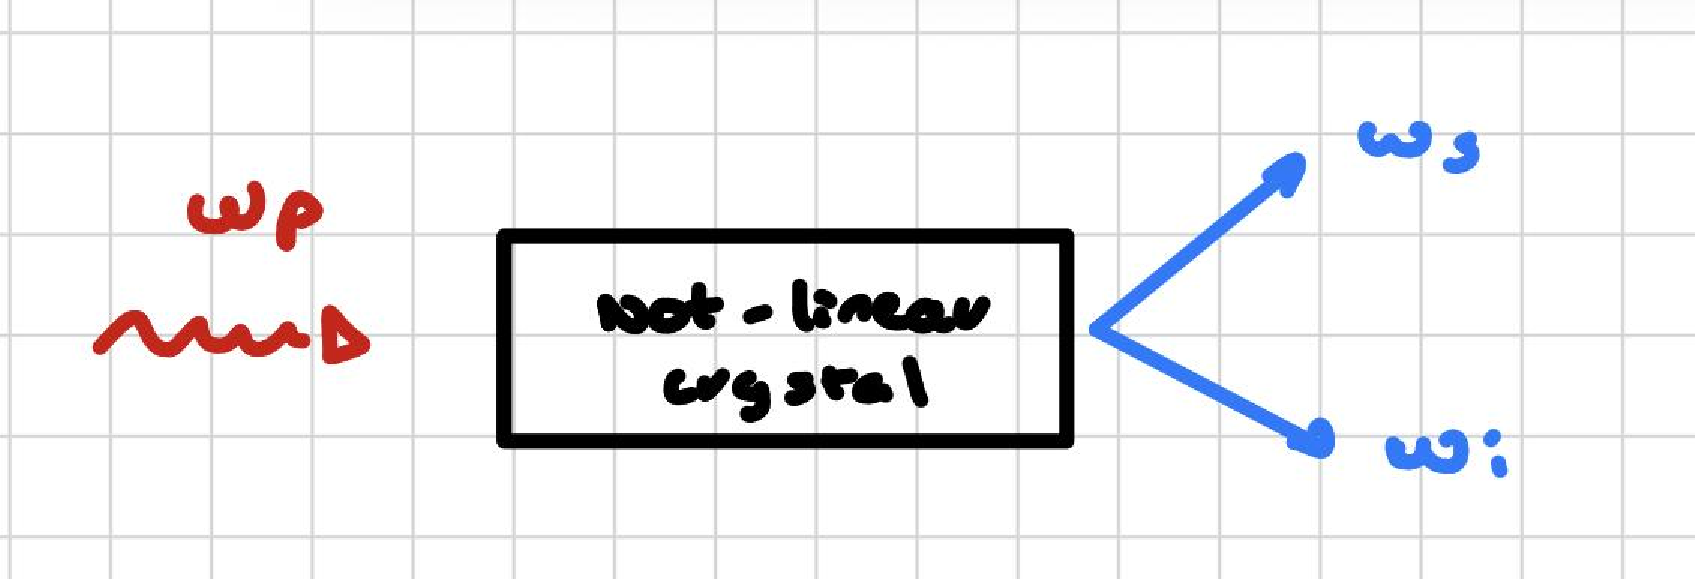
\includegraphics[width=0.6\linewidth]{images_in_pdf/16-/Grafico_86.pdf}
\end{figure}

We assume that the \hl{pump field is quantized} and the interaction Hamiltonian have the form:
\begin{equation}\label{eqn:16-interaction-hamiltonian}
\hat{H} \propto \chi^{(2)}\, \hat{a}_p\, \hat{a}_s^+\, \hat{a}_i^+ 
\end{equation}

Where \hl{$\chi^{(2)}$ is the second order non-linear susceptibility} and it cames from the polarization when we consider non-centrosymmetric crystals:
\begin{equation}\label{eqn:16-polarization-non-linear}
\vec{P} = \epsilon_0 \, \chi \, \vec{E}+ \epsilon_0 \, \chi^{(2)}\, \vec{E}^2+...
\end{equation}

\hl{$\hat{a}_p$ is the annihilation operator of the pump beam, $\hat{a}_s^+$ is the creation operator for the signal and $\hat{a}_i^+$ is the creation operator for the idler wave}.

Initially we have a sigle photon state for the pump, joint with a vacuum state for signal and idler, then we obtain through a \textbf{spontaneous process:}
\begin{equation}\label{eqn:16-spontaneous-process}
\hat{a}_p\, \hat{a}_s^+\, \hat{a}_i^+ \, \ket{1}_p\ket{0}_s\ket{0}_i = \ket{0}_p\ket{1}_s\ket{1}_i
\end{equation}

In order to obtain it we we need to satisfy some requirements called \textbf{Phase matching conditions}:
\begin{itemize}
    \item \emph{Conservation of energy}:
    \begin{equation}\label{eqn:16-phase-matching-energy}
    \hbar \omega_p = \hbar\omega_s+\hbar\omega_i
    \end{equation}

    \item \emph{Conservation of momentum}:
    \begin{equation}\label{eqn:16-phase-matching-momentum}
    \hbar \vec{k}_p =\hbar \vec{k}_s+\hbar \vec{k}_i
    \end{equation}
\end{itemize}

Typically we use a UV photon and obtain two IR photons, notice that to satisfy them also the direction of the beam is important.

\calloutinfo{%
    In the so called \textbf{Type II} crystals the polarizations of signal and idler photons are orthogonal, this makes it possible to generate \textbf{entangled states}:
\begin{equation}\label{eqn:16-entangled-state}
\ket{\psi} = \frac{1}{\sqrt{2}}\, 
\bigl[ 
    \ket{H}_s\ket{V}_i+\ket{V}_s\ket{H}_i
\bigr]
\end{equation}

In case instead of a \textbf{Type I} crystal, the polarizations of signal and idler are the same: we don't obtain entangled photons, but it can be useful in order to have a indistinguishable photon source.
}

\subsection{Interference experiments}
We are interested in understanding what happens if our twin single photons are simultaneously incident at each input port of a B.S.

We need to describe the B.S. with quantum mechanics: 
\begin{figure}[H]
    \centering
    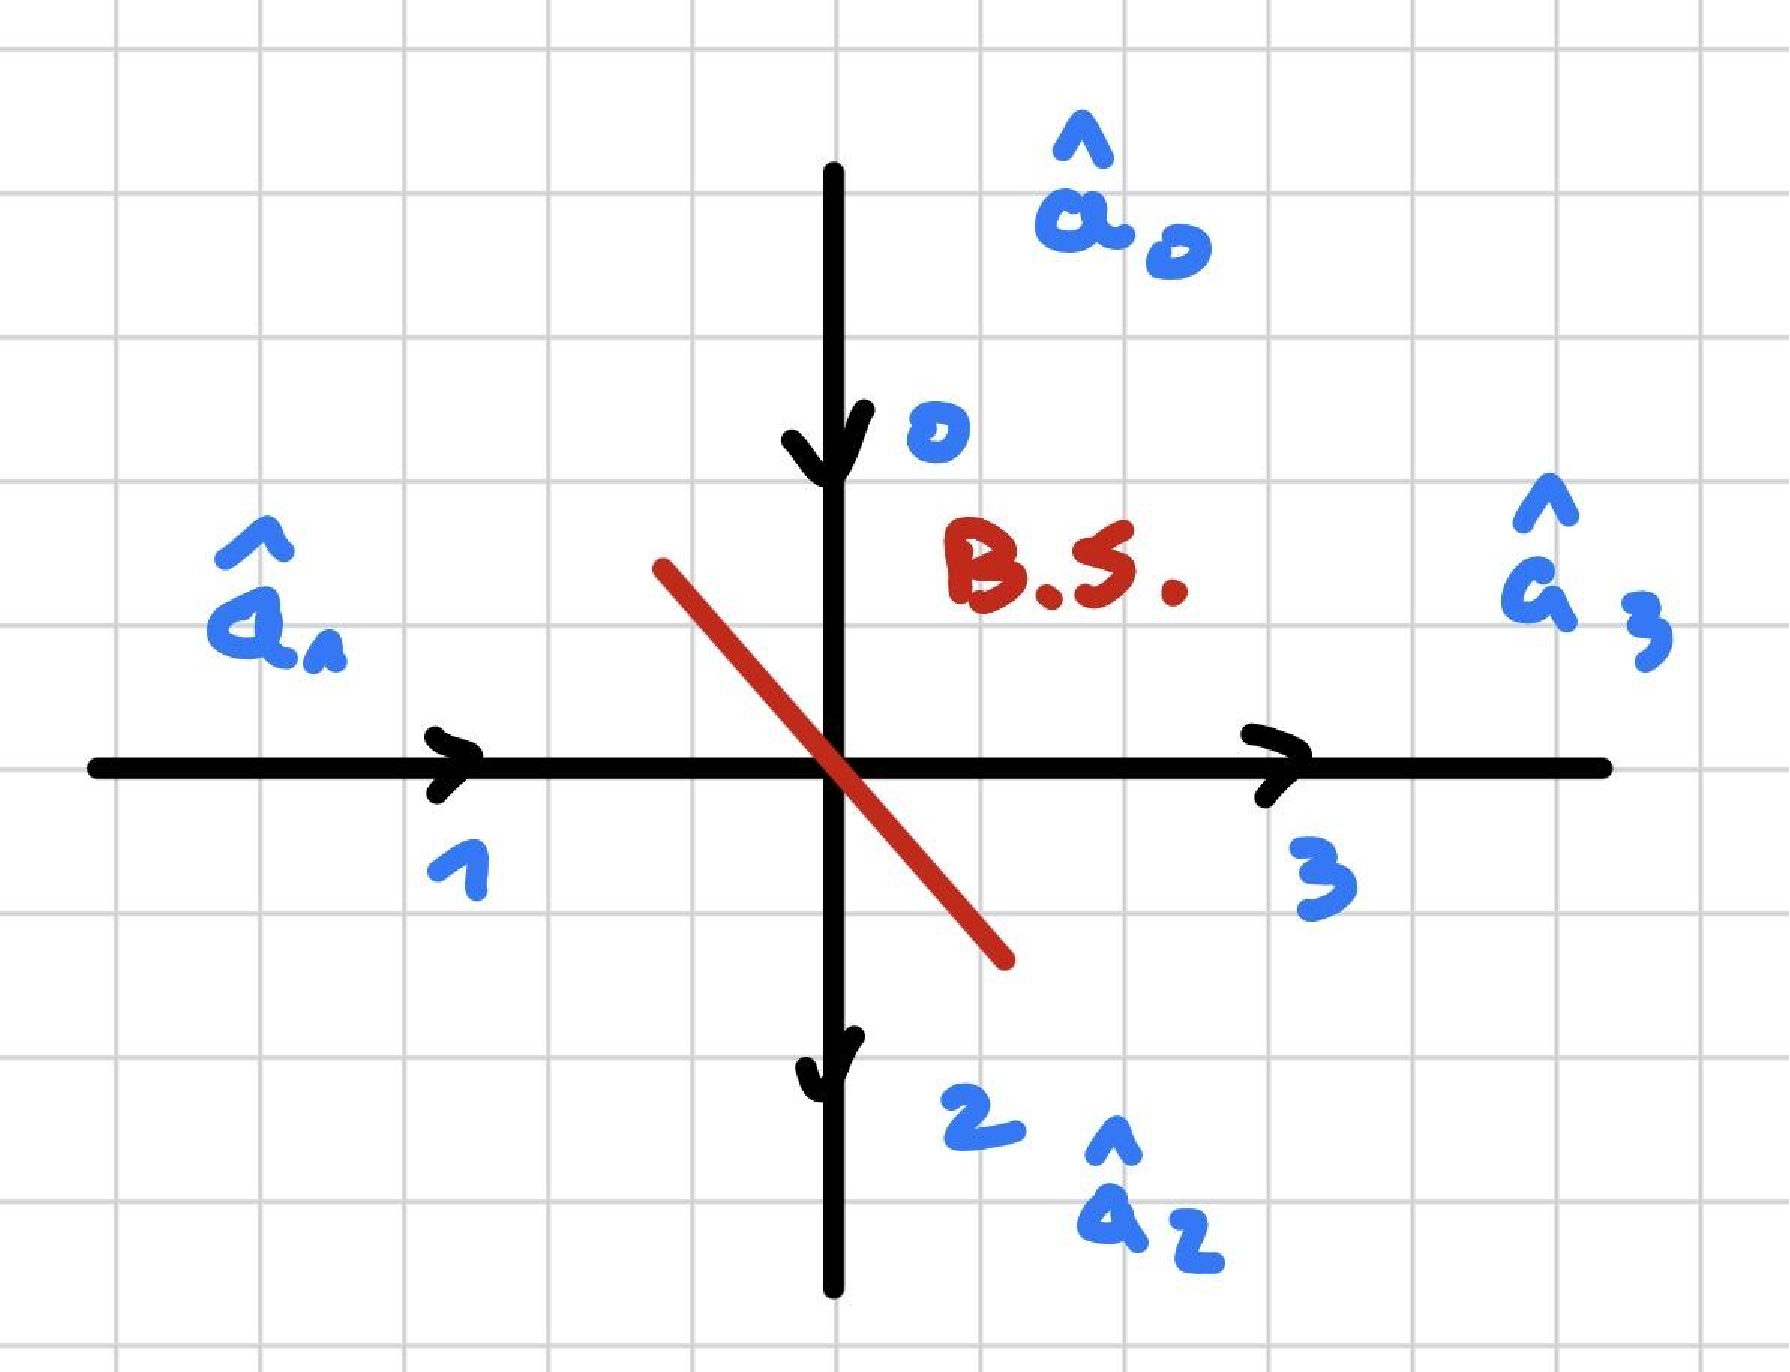
\includegraphics[width=0.6\linewidth]{images_in_pdf/16-/Grafico_87.pdf}
\end{figure}

Let's consider a B.S. with two input ports $1$ and $0$ and two exit ports $2$ and $3$, for each we can associate an annihilation operator $\hat{a}_i$.

If $\refl$ and $\tran$ are the complex \textbf{reflectance} and \textbf{transmittance} of the beam splitter B.S., \hl{from the classical point of view we send an electric field $E_1$ which is transmitted as $E_3$ and reflected as $E_2$}:
\begin{equation}\label{eqn:16-classical-b-s}
\begin{cases}
    E_2 = \refl\, E_1\\[0.5ex]
    E_3 = \tran\, E_1
\end{cases}
\end{equation}

Where $E_i$ stands for the complex amplitude of the light field; for a $50:50$ B.S. we will obtain:
\begin{equation}\label{eqn:16-50-50-b-s}
\begin{cases}
    |\refl| = |\tran| = \frac{1}{\sqrt{2}}\\[0.5ex]
    |\refl|^2 + |\tran|^2 =1
\end{cases}
\end{equation}

\hl{According to quantum mechanics, we must consider the equivalent coefficients $\refl,\tran \to \refl',\tran'$ for the input port $0$ which correspond to a vacuum state}:
\begin{equation}\label{eqn:16-quantum-b-s}
\begin{cases}
    \hat{a}_2 = \refl\,\hat{a}_1+\tran'\,\hat{a}_0\\[0.5ex]
    \hat{a}_3 = \tran\, \hat{a}_1+\refl'\, \hat{a}_0
\end{cases}\implies \begin{pmatrix}
    \hat{a}_2\\[0.5ex]
    \hat{a}_3
\end{pmatrix} = \begin{pmatrix}
    \refl' &\tran\\[0.5ex]
    \tran' &\refl
\end{pmatrix}\begin{pmatrix}
    \hat{a}_0\\[0.5ex]
    \hat{a}_1
    \end{pmatrix}
\end{equation}

For a $50:50$ B.S. reflected and transmitted beams have the same amplitude, but they are different in phase:
\begin{equation}\label{eqn:16-50-50-b-s-phase}
\begin{cases}
    \hat{a}_2= \frac{1}{\sqrt{2}}\, 
    \left( \hat{a}_0+i\hat{a}_1\right)\\[0.5ex]
    \hat{a}_3= \frac{1}{\sqrt{2}}\, 
    \left( i\hat{a}_0+\hat{a}_1\right)
\end{cases}
\end{equation}

\subsubsection{One photon and vacuum state at the input ports}

Let's discuss the case where we have a single photon arriving at the input port $1$, so that the two initial states can be rewritten as functions of the creation operators:
\begin{equation}\label{eqn:16-single-photon-state}
\ket{0}_0\ket{1}_1 = \hat{a}_1^\dagger \, \ket{0}_0\ket{0}_1
\end{equation}

From previous equations and taking the dagger, we can rewrite:
\begin{equation}\label{eqn:16-b-s-creation-operators}
\begin{split}
\hat{a}_3^\dagger +i\hat{a}_2^\dagger  &= \frac{1}{\sqrt{2}}
\bigl[
    -i\hat{a}_0^\dagger +\hat{a}_1^\dagger +i(\hat{a}_0^\dagger -i\hat{a}_1^\dagger )
\bigr] = \\[0.5ex]
&= \frac{1}{\sqrt{2}}
\bigl[
    \cancel{-i\hat{a}_0^\dagger }+\hat{a}_1^\dagger +\cancel{i\hat{a}_o^+}+\hat{a}_1^\dagger 
\bigr] = \\[0.5ex]
&= \frac{1}{\sqrt{2}} \, 2\hat{a}_1^\dagger \\[0.5ex]
\iff \hat{a}_1^\dagger  &= \frac{1}{\sqrt{2}}(\hat{a}_3^\dagger +i\hat{a}_2) 
\end{split}
\end{equation}

Notice also that the action of B.S. on vacuum state entering input port gives as result: 
\begin{equation}\label{eqn:16-vacuum-state}
\ket{0}_0\ket{0}_1 \mapsto \ket{0}_2\ket{0}_3
\end{equation}

So we can substitute and obtain:
\begin{equation}\label{eqn:16-single-photon-state-2}
\ket{0}_0\ket{1}_1 = \frac{1}{\sqrt{2}} (i\hat{a}_2^\dagger +\hat{a}_3^\dagger ) \, \ket{0}_2\ket{0}_3 = 
\frac{1}{\sqrt{2}}\, 
\left(
    i\ket{1}_2\ket{0}_3+ \ket{0}_2\ket{1}_3
\right)
\end{equation}

\calloutinfo{%
    We obtained an \textbf{entangled state} between output ports $2$ and $3$, we cannot have coincidence counts! We can have 1 photon only in one arm and never  simultaneously in both.
} 
When we measure one of the two arms we collapse the wave function and destroy the interference.

\subsubsection{Two photons at the input ports}

Let's come back and study the case of twin single photons injected into two ports of the B.S.:

\begin{figure}[H]
    \centering
    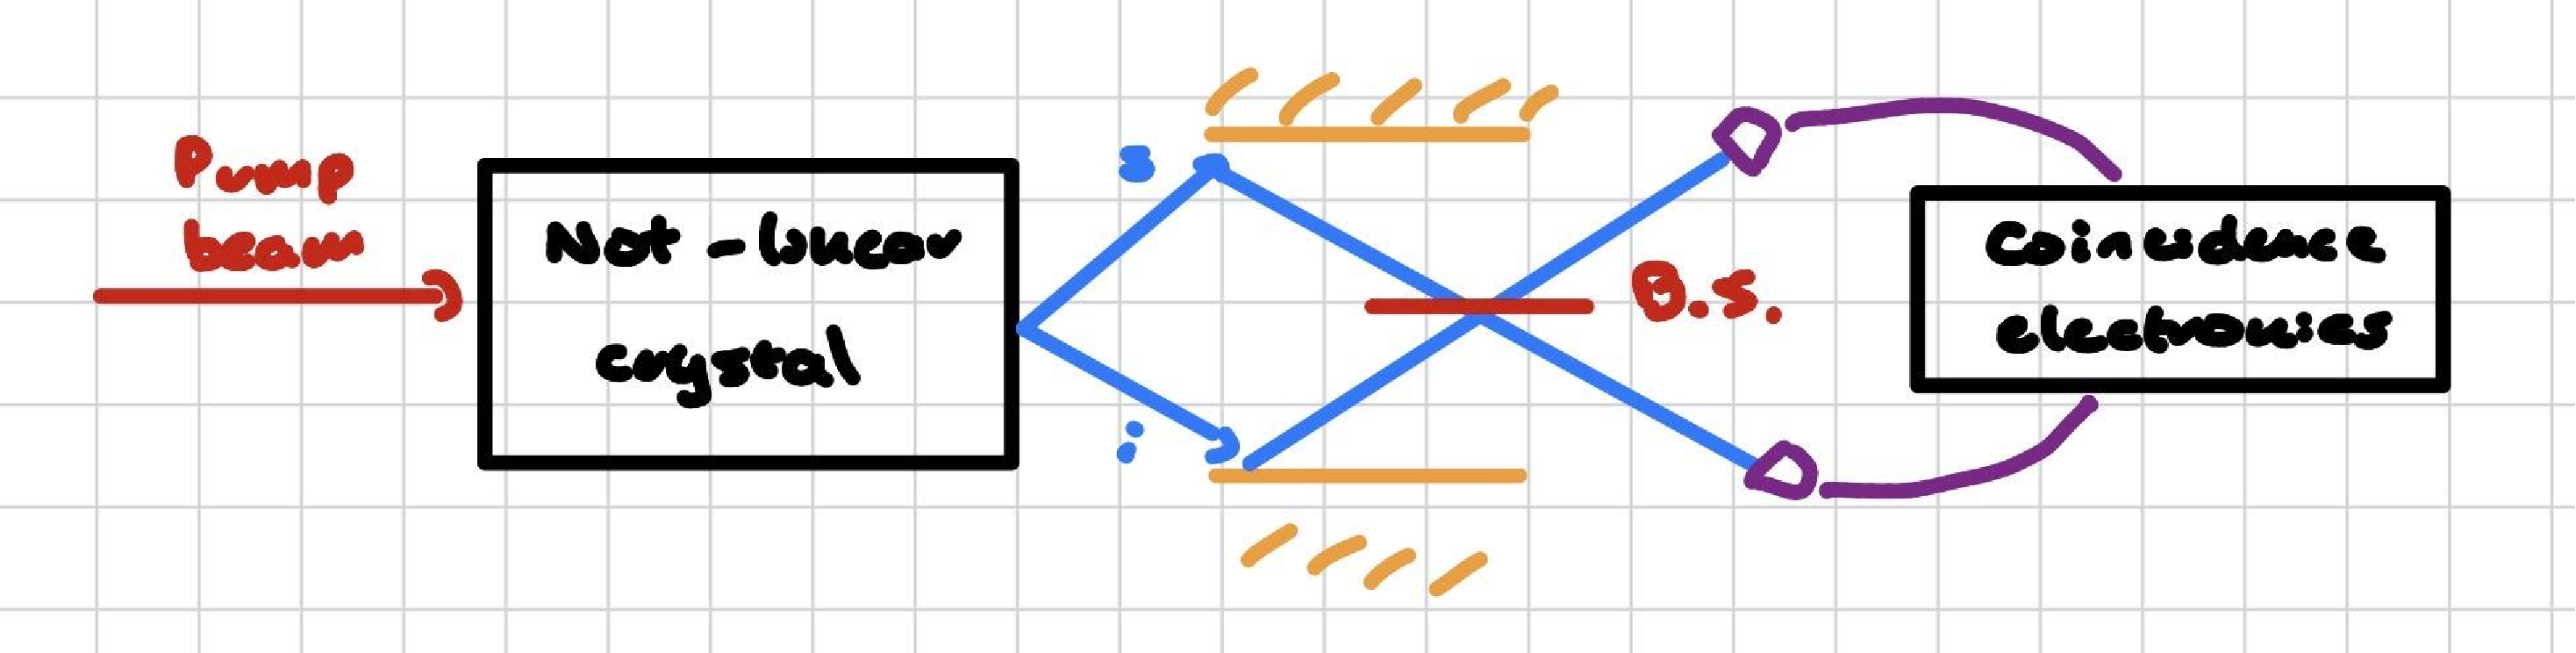
\includegraphics[width=0.6\linewidth]{images_in_pdf/16-/Grafico_88.pdf}
\end{figure}
\begin{figure}[H]
    \centering
    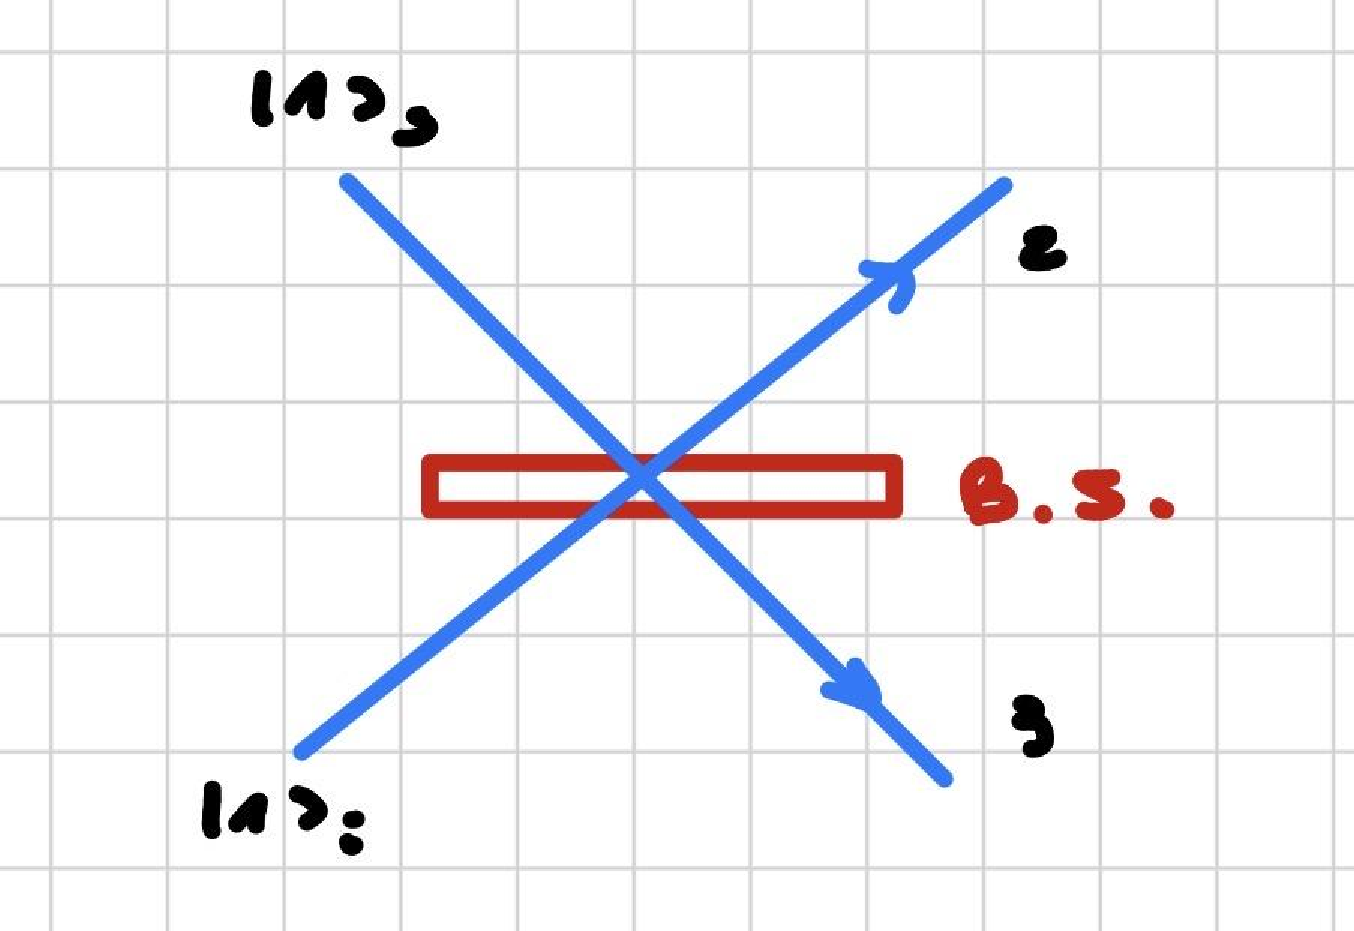
\includegraphics[width=0.6\linewidth]{images_in_pdf/16-/Grafico_89.pdf}
\end{figure}

The pump beam excites a nonlinear crystal, which emits pairs of photons, usually referred to as \textbf{signal} ($s$) and \textbf{idler} ($i$). After removing the pump, the two photons are reflected by mirrors and sent to the two input ports of a balanced beam splitter (BS). The output fields are then collected by two detectors connected to a coincidence circuit in order to perform the measurement.

We send the states $\ket{1}_s$ and $\ket{1}_i$ into the BS. 

\textbf{What should we expect at the output ports?}

As in the previous case, we can rewrite the initial state as
\begin{equation}\label{eqn:16-twin-single-photon-state}
\ket{1}_0\ket{1}_1 = \hat a_0^\dagger \hat a_1^\dagger \ket{0}_0\ket{0}_1,
\end{equation}

where the beam splitter transformation for the creation operators is
\begin{equation}\label{eqn:16-b-s-creation-operators-2}
\begin{cases}
\hat a_0^\dagger = \frac{1}{\sqrt{2}}\left(\hat a_2^\dagger + i\hat a_3^\dagger\right),\\[1ex]
\hat a_1^\dagger = \frac{1}{\sqrt{2}}\left(i\hat a_2^\dagger + \hat a_3^\dagger\right).
\end{cases}
\end{equation}

Moreover, the vacuum is mapped as
\begin{equation}\label{eqn:16-vacuum-state-mapping}
\ket{0}_0\ket{0}_1 \to \ket{0}_2\ket{0}_3.
\end{equation}

Therefore,
\begin{equation}\label{eqn:16-single-photon-state-3}
\begin{split}
    \implies \ket{1}_0\ket{1}_1 &= 
    \frac{1}{\sqrt{2}}\frac{1}{\sqrt{2}}
    \left(\hat{a}_2^\dagger +i\hat{a}_3^\dagger \right)\, 
    \left(i\hat{a}_2^\dagger +\hat{a}_3^\dagger \right)\, 
    \ket{0}_2\ket{0}_3 = \\[0.5ex]
    &=\frac{i}{2}
    \left(\hat{a}_2^\dagger \hat{a}_2^\dagger +\hat{a}_3^\dagger \hat{a}_3^\dagger \right) \ket{0}_2\ket{0}_3 \propto \\[0.5ex]
    &\propto i\,
    \bigl(\ket{2}_2\ket{0}_3+\ket{0}_2\ket{2}_3\bigr) 
    = \ket{\psi}_{B.S.}
\end{split}
\end{equation}

The disappearance of the central terms in the expansion is a direct consequence of both the bosonic nature of photons and the phase relations introduced by the beam splitter. The mixed terms $\hat a_2^\dagger \hat a_3^\dagger$ and $\hat a_3^\dagger \hat a_2^\dagger$ correspond to the configuration in which one photon exits each output port, i.e. the state $\ket{1}_2\ket{1}_3$. Since photons are bosons, operators acting on different ports commute, $\hat a_2^\dagger \hat a_3^\dagger = \hat a_3^\dagger \hat a_2^\dagger$, and these two contributions cancel exactly due to their opposite relative phase. As a result, \hl{the coincidence term vanishes}.

\hl{This implies that both photons always leave the beam splitter through the same output port}. This behavior cannot be understood within a classical picture based on independent trajectories, but arises from quantum interference between indistinguishable processes. 
In particular, there are two possible ways to obtain a coincidence event: 
\begin{enumerate}
\item Both photons being transmitted;
\item Both photons being reflected.
\end{enumerate}

\hl{Since these processes are indistinguishable, their probability amplitudes must be summed before taking the modulus squared}, leading to \textbf{destructive interference} and a vanishing coincidence probability.

Defining the transmission and reflection amplitudes as
\begin{equation}\label{eqn:16-b-s-amplitudes}
A_\tran = \frac{1}{\sqrt{2}}, \qquad A_\refl = \frac{i}{\sqrt{2}},
\end{equation}

the coincidence amplitude is
\begin{equation}\label{eqn:16-coincidence-amplitude}
A_\tran A_\tran + A_\refl A_\refl = \frac{1}{2} + \frac{i^2}{2} = 0,
\end{equation}

and therefore
\begin{equation}\label{eqn:16-coincidence-probability}
P_{11} = \left|A_\tran A_\tran + A_\refl A_\refl\right|^2 = \left|\frac{1}{\sqrt{2}}\frac{1}{\sqrt{2}}+\frac{i}{\sqrt{2}}\frac{i}{\sqrt{2}}\right|^2 = 0
\end{equation}

\calloutinfo{%
    In the ideal case, coincidences are completely suppressed, and the output state is a two-photon bunched state.
    This effect cannot be interpreted classically; it is a direct consequence of two-photon interference and bosonic symmetry.
}

\subsubsection{Hong-Ou-Mandel proof-of-principle experiment}

In 1982, Hong, Ou, and Mandel demonstrated two-photon interference using a \textbf{type-I nonlinear crystal} with the setup shown below. The pump beam excites the crystal and generates correlated photon pairs, conventionally called signal ($s$) and idler ($i$); the pump is then removed by a mirror or a suitable filter, while the two photons are spectrally selected with a B.S. and sent along two paths whose optical lengths can change by moving the position of the B.S. In this way, one introduces a relative delay
\begin{equation}\label{eqn:16-relative-delay}
\Delta\tau = \tau_s - \tau_i,
\end{equation}

between the two photons. The outputs of the beam splitter are detected by two photodetectors connected to a coincidence counter, so that the coincidence rate can be measured as a function of the relative delay.

\begin{figure}[H]
    \centering
    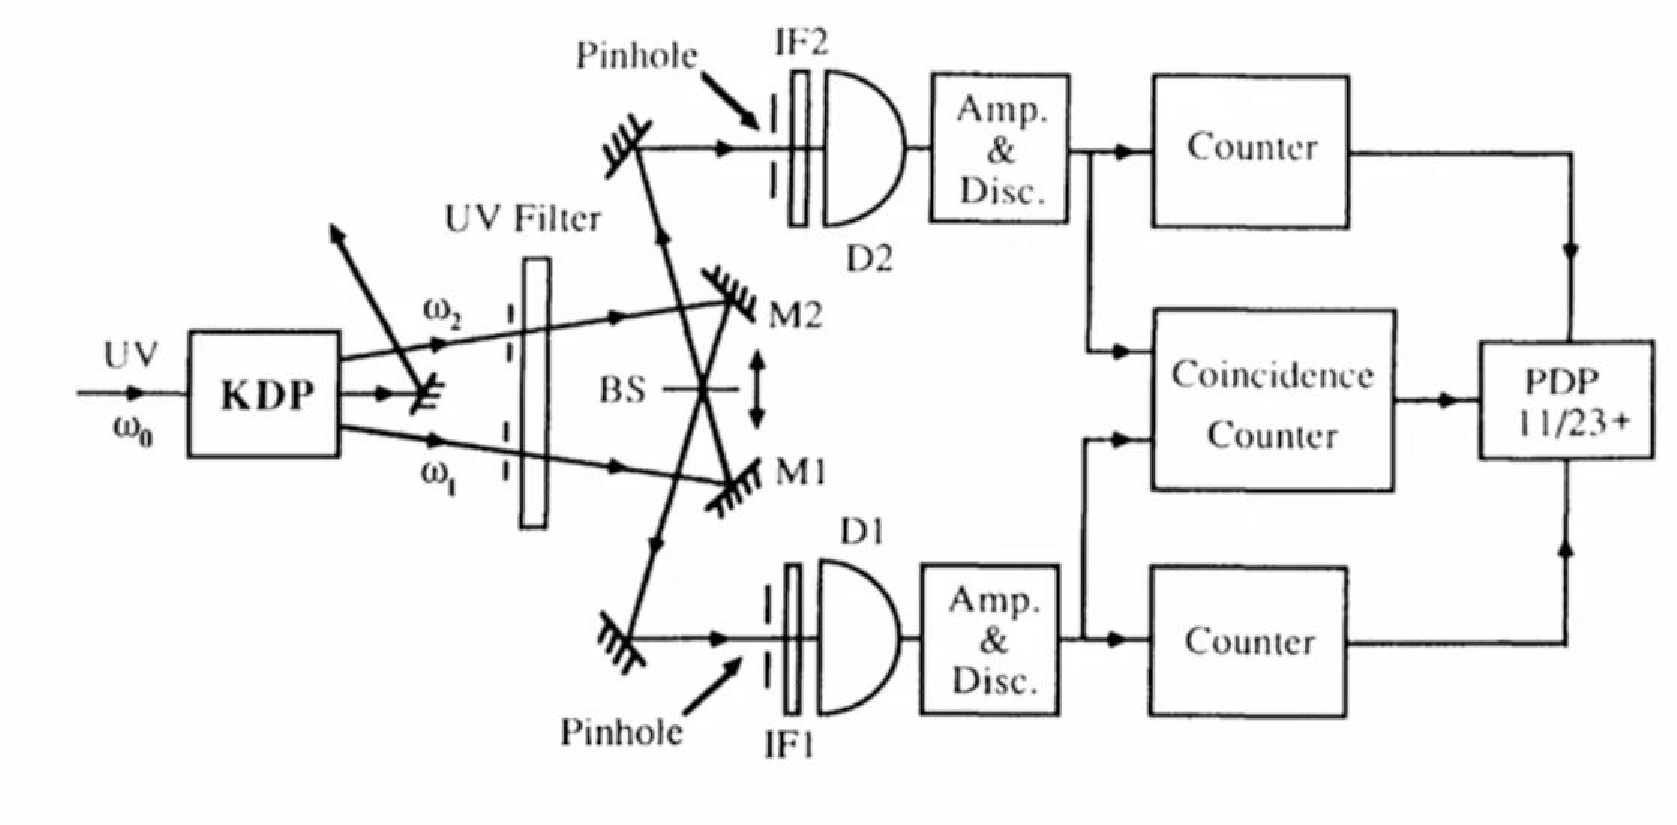
\includegraphics[width=0.9\linewidth]{images_in_pdf/16-/Grafico_90.pdf}
    \caption{Hong-Ou-Mandel interference set-up.}
    \label{fig:esempio}
\end{figure}

\begin{itemize}
    \item \hl{When $\Delta\tau = 0$}, the two wave packets overlap at the beam splitter and, if the photons are indistinguishable, the coincidence rate ideally drops to zero: this is the Hong--Ou--Mandel effect. This does not mean that the photons simply travel through one arm or the other in a classical sense; rather, \hl{the vanishing of coincidences is a genuine quantum interference effect arising from two indistinguishable two-photon amplitudes}, namely the case in which both photons are transmitted and the case in which both are reflected.
    
    \item \hl{For large delays, $|\Delta\tau| \gg \tau_c$}, where the coherence time is of order $\tau_c \sim 1/\Delta\omega$, \hl{the overlap between the two photons disappears}, the interference term vanishes, and the coincidence rate returns to the classical level: \hl{this happens because the two photons are no longer indistinguishable!}. For an ideal balanced beam splitter this corresponds to a normalized value of $1/2$.

\end{itemize}
\begin{figure}[H]
    \centering
    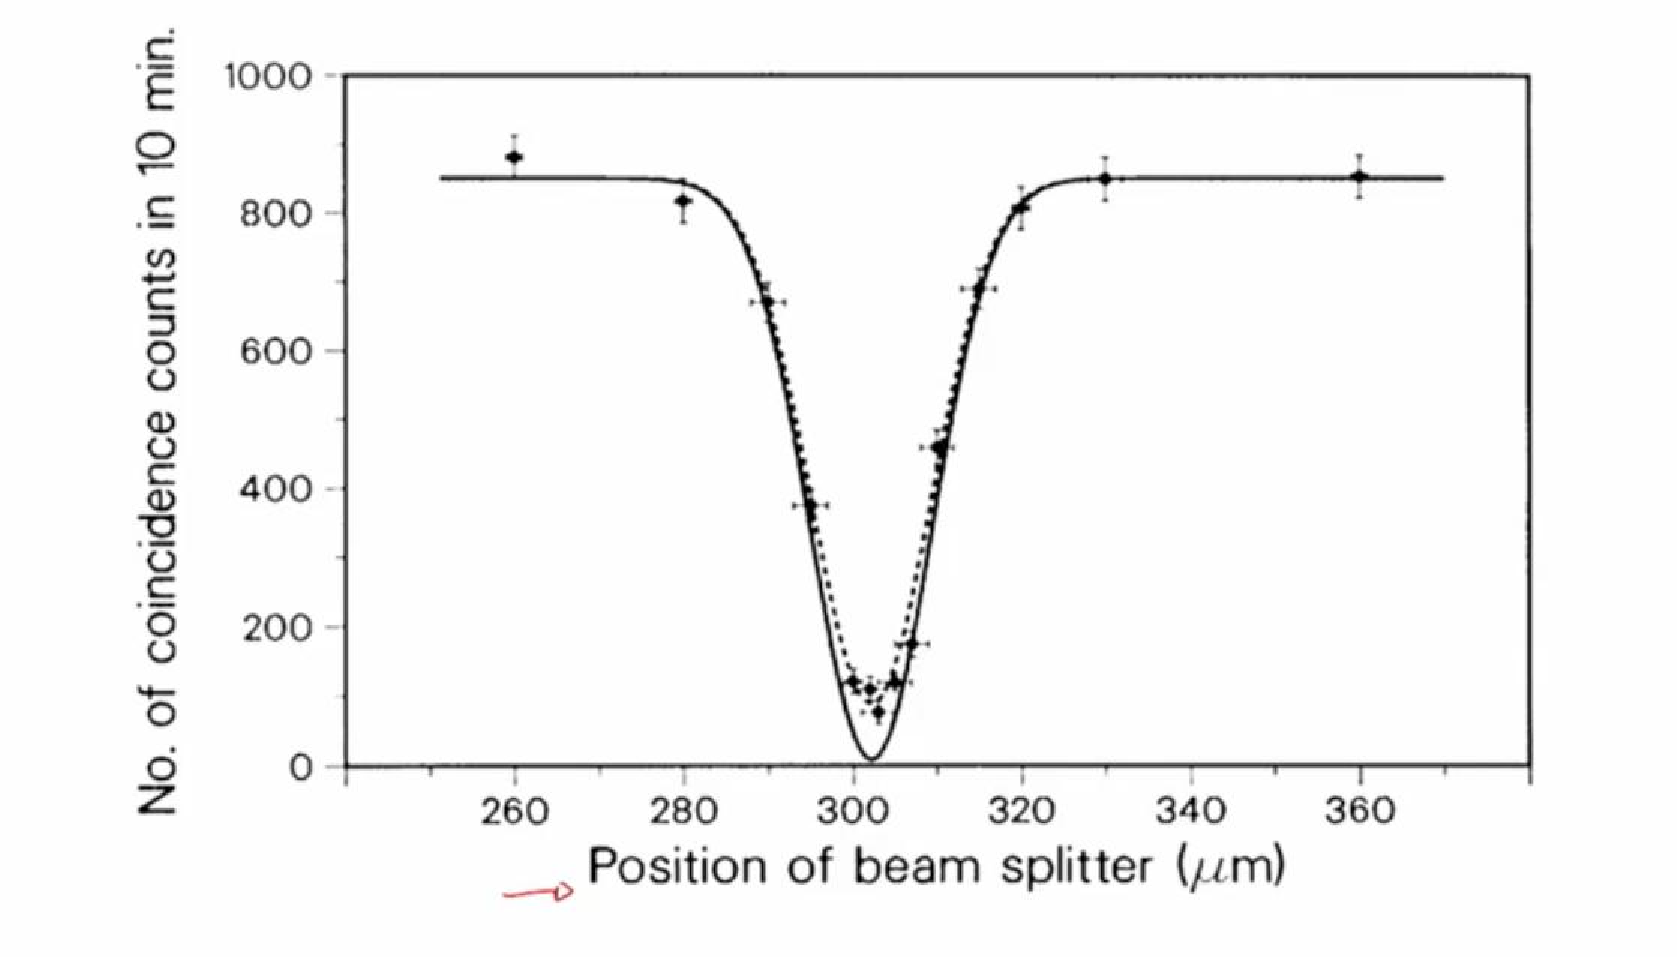
\includegraphics[width=0.9\linewidth]{images_in_pdf/16-/Grafico_91.pdf}
    \caption{Coincidence rate as a function of the relative delay $\Delta\tau$. The dip at zero delay is a signature of two-photon interference.}
    \label{fig:esempio2}
\end{figure}

\calloutinfo{%
    Notice that $\tau_c \approx ns$ which is difficult to measure by using time resolved detectors, by using this interferometer we can measure precisely the width of the dip which provides a direct measure of the temporal coherence of the photon wave packets.
}

\subsection{Quantum Eraser}

Suppose we consider the same system as before, but \hl{now we insert a half-wave plate along the idler arm}. This changes the polarization of the idler photon and, therefore, introduces a polarization tag that can carry which-path information:
\begin{figure}[H]
    \centering
    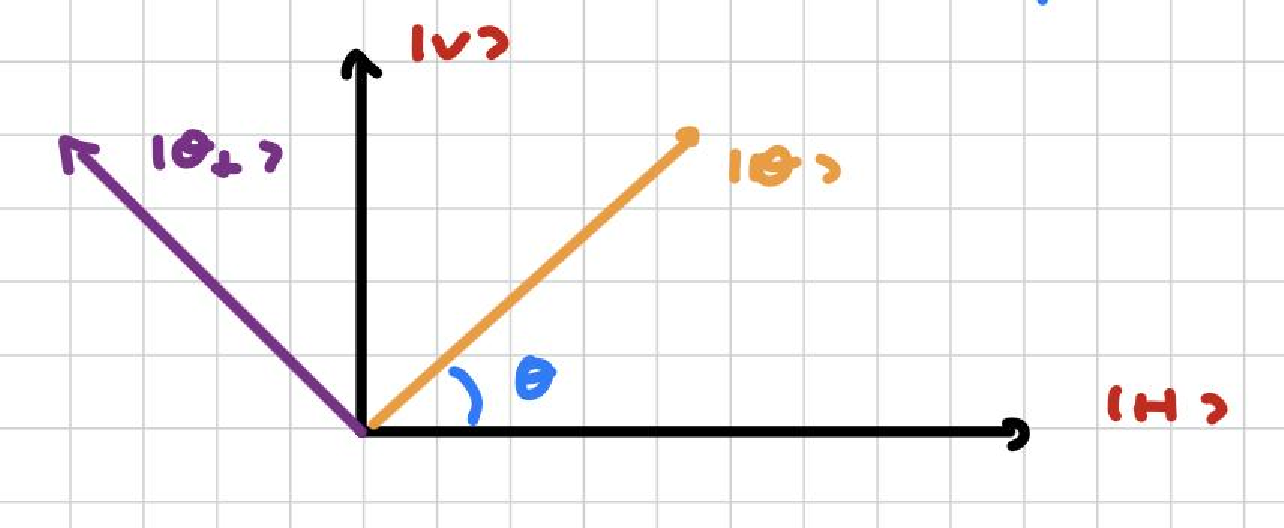
\includegraphics[width=0.6\linewidth]{images_in_pdf/16-/Grafico_92.pdf}
\end{figure}

\begin{equation}\label{eqn:16-polarization-states}
\ket{\theta}_i = 
\cos(\theta)\ket{H}_i + \sin(\theta)\ket{V}_i,
\qquad
\ket{\theta_\perp}_i = 
-\sin(\theta)\ket{H}_i + \cos(\theta)\ket{V}_i .
\end{equation}

If the original polarization of the signal photon is horizontal $\ket{H}$, the input state is no longer simply \(\ket{H}_s\ket{H}_i\), but rather
\begin{equation}\label{eqn:16-tagged-polarization}
    \ket{H}_s\ket{\theta}_i = \cos(\theta)\,\ket{H}_s\ket{H}_i + \sin(\theta)\, \ket{H}_s\ket{V}_i
\end{equation}

Using the same beam-splitter transformation as before, the output state is no longer the purely bunched two-photon state:
\begin{equation}\label{eqn:16-output-state}
    \ket{\psi}_{output} = \frac{i}{\sqrt{2}}\, \ket{0}_2\ket{2H}_3+\frac{i}{\sqrt{2}}\, \ket{2H}\ket{0}_3
\end{equation}

but instead becomes 
\begin{equation}\label{eqn:16-output-state-tagged}
\begin{split}
    \ket{\psi(\theta)}_{output} &= 
    \frac{i}{\sqrt{2}}\, \cos(\theta)\, 
    \bigl(
        \ket{2H}_2\ket{0}_3+\ket{0}_2\ket{2H}_3
    \bigr) + \\[0.5ex]
    &+\frac{1}{2}\, \sin(\theta)\, 
    \bigl(
        \ket{H}_2\ket{V}_3-\ket{V}_2\ket{H}_3
    \bigr) + \\[0.5ex]
    &+\frac{i}{2}\, \sin(\theta)\, 
    \bigl(
        \ket{H,V}_2\ket{0}_3-\ket{0}_2\ket{H,V}_3
    \bigr)
\end{split}
\end{equation}

\hl{When $\theta = \pi/2$, the idler photon becomes vertically polarized, while the signal photon remains horizontally polarized}. The two photons are therefore orthogonal in polarization and become distinguishable. The output state can be written as
\begin{equation}\label{eqn:16-output-state-orthogonal}
\Ket{\psi\!\left(\frac{\pi}{2}\right)}_{\text{output}}
=
\underbrace{\frac{1}{2}\bigl(\ket{H}_2\ket{V}_3-\ket{V}_2\ket{H}_3\bigr)}%
_{\Rnum{1}}
+
\underbrace{\frac{i}{2}\bigl(\ket{H,V}_2\ket{0}_3-\ket{0}_2\ket{H,V}_3\bigr)}%
_{\Rnum{2}}.
\end{equation}

\begin{enumerate}
    \item The first term ($\Rnum{1}$) describes events in which the two photons exit through different output ports, leading to coincidence detections;
    \item The second term ($\Rnum{2}$) corresponds to both photons exiting through the same output port with orthogonal polarizations. 
\end{enumerate}

\calloutwarn{%
Since the photons are distinguishable, the two-photon interference responsible for the Hong--Ou--Mandel effect is no longer complete, and \textbf{coincidence counts reappear}.

Physically, \textbf{the polarization degree of freedom carries which-path information}, allowing one in principle to distinguish the two photons, thereby reducing the destructive interference. 
} 

\begin{figure}[H]
    \centering
    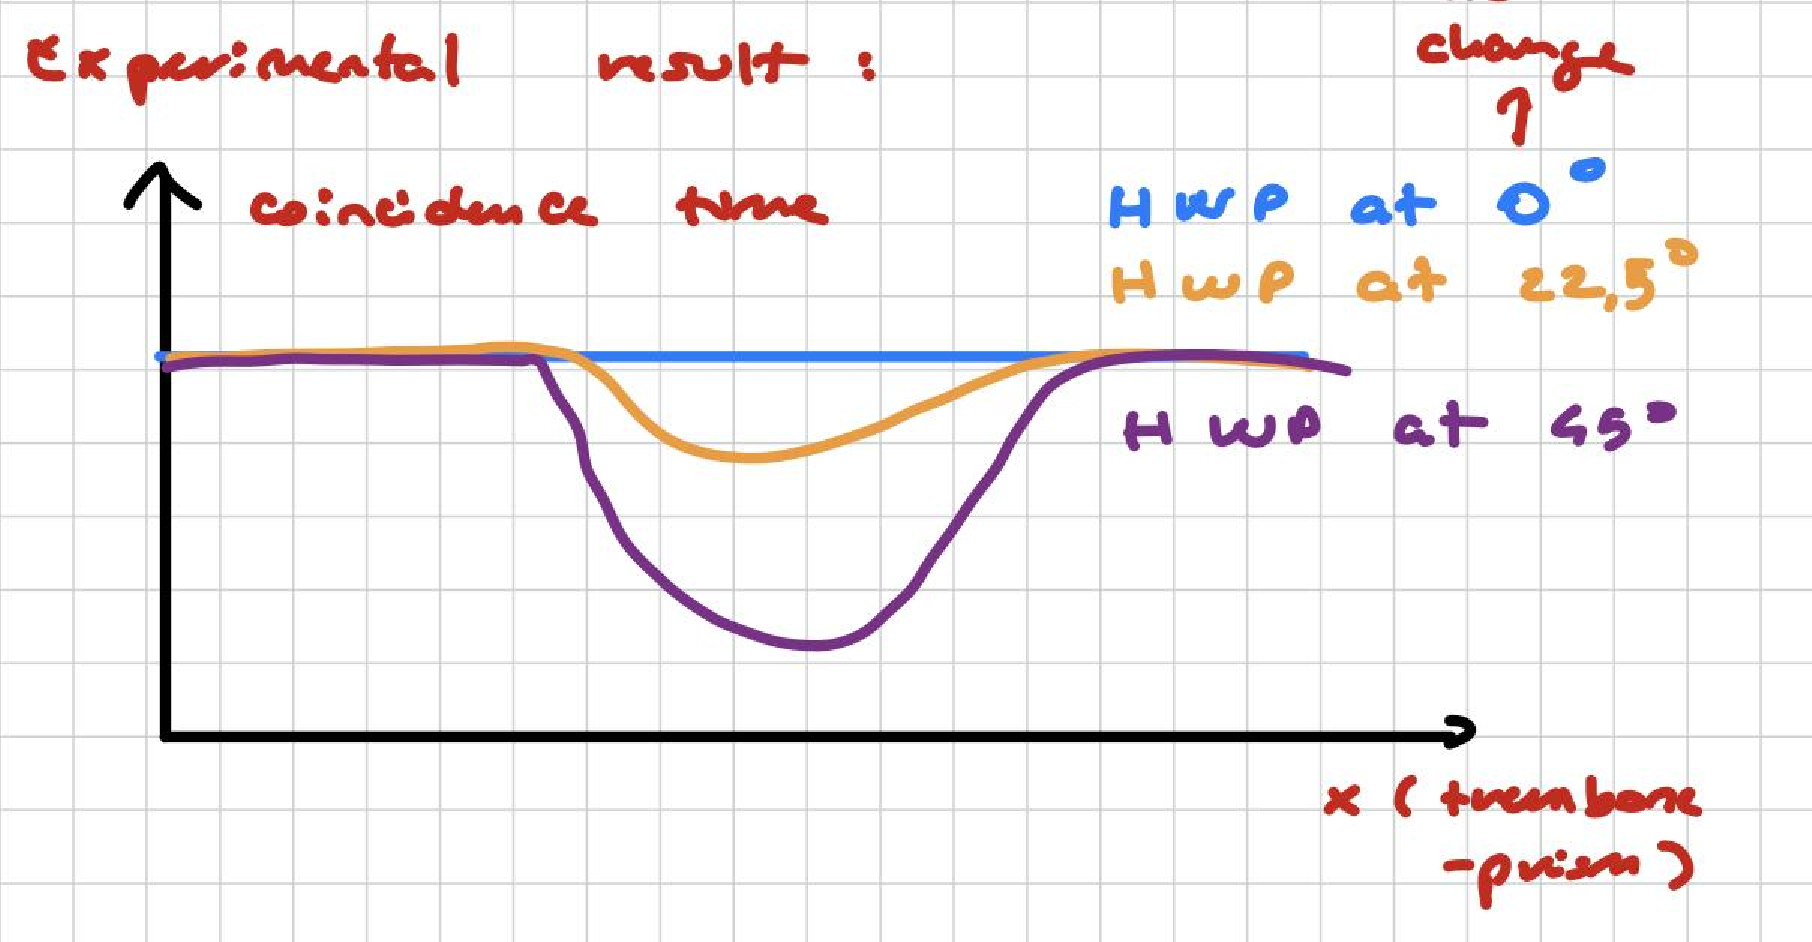
\includegraphics[width=0.6\linewidth]{images_in_pdf/16-/Grafico_93.pdf}
\end{figure}
\textbf{However}, \hl{the information is erased if both output beams are projected onto the same polarization basis by placing polarizers before the detectors} with $\theta_a$ and $\theta_b$. In that case, the coincidence probability becomes
\begin{equation}\label{eqn:16-coincidence-probability-erased}
P = \left|\bra{\theta_a}\braket{\theta_b | \psi_{\text{output}}}\right|^2
= \frac{1}{4}\sin^2(\theta_b-\theta_a),
\end{equation}

so that $P\to 0$ when $\theta_a=\theta_b$.

This restores indistinguishability in the selected sub-ensemble and is the essence of the quantum eraser.
\begin{figure}[H]
    \centering
    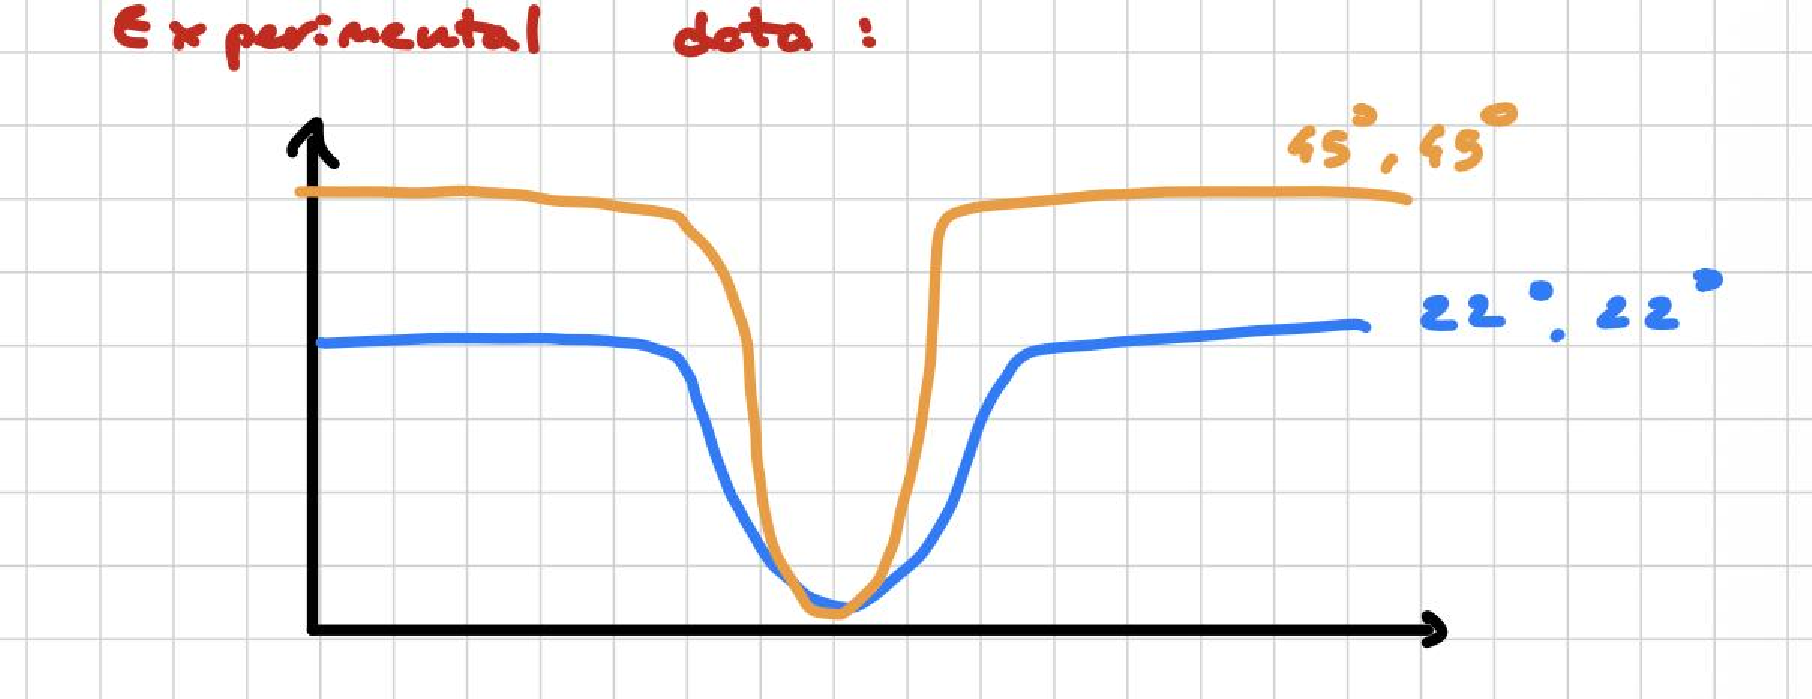
\includegraphics[width=0.6\linewidth]{images_in_pdf/16-/Grafico_94.pdf}
    \caption{Intensity measurements at \qty{45}{\degree} and \qty{22}{\degree}}
\end{figure}

\subsection{Application of entanglement to interferometry}
Classically, the measurement of the difference photocurrent in an interferometer exhibits a sinusoidal fringe pattern when a phase shift is introduced by an optical element in one arm. 

\begin{figure}[H]
    \centering
    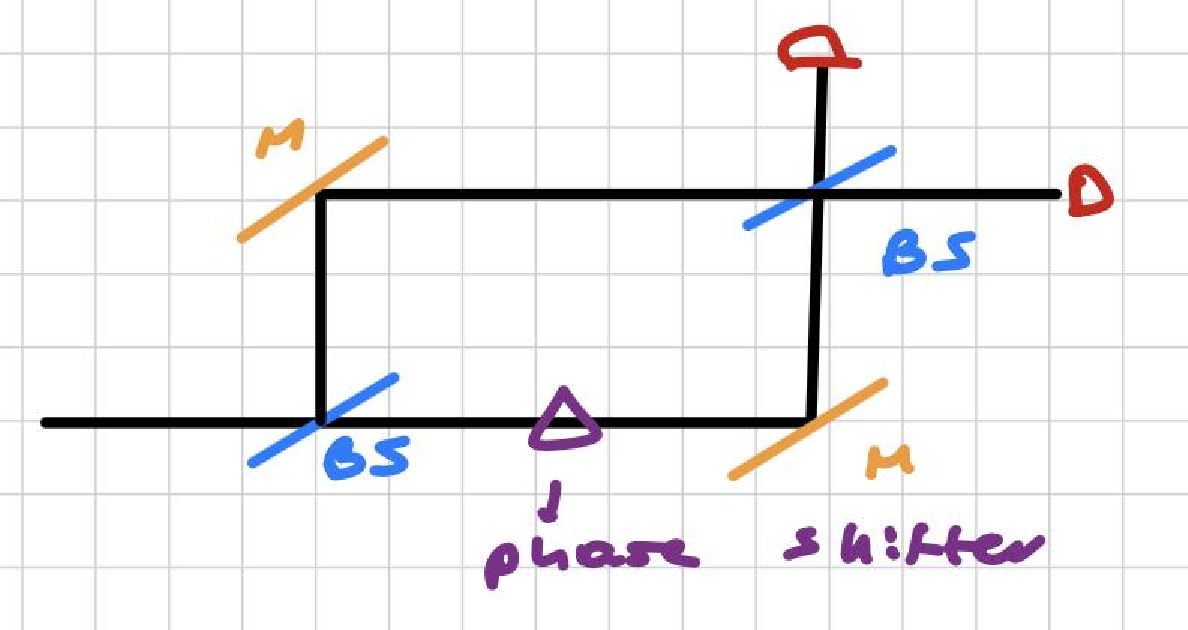
\includegraphics[width=0.6\linewidth]{images_in_pdf/16-/Grafico_95.pdf}
\end{figure}

The accuracy of the phase measurement $\Delta\theta$ is limited by photocurrent fluctuations, namely shot noise. For an input beam with mean photon number $\bar n$, the standard quantum limit gives
\begin{equation}\label{eqn:16-shot-noise-limit}
\Delta\theta \sim \frac{1}{\sqrt{\bar n}}.
\end{equation}

As in applications such as gravitational-wave detection, the \hl{phase sensitivity can be improved by using non-classical light}. Consider now one photon entering each input port of the first beam splitter:
\begin{figure}[H]
    \centering
    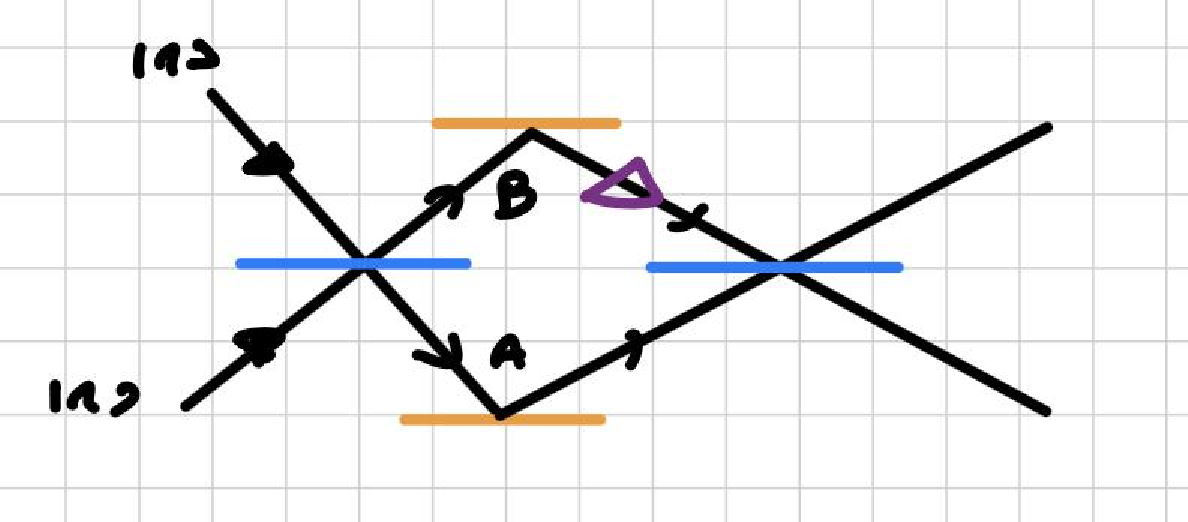
\includegraphics[width=0.6\linewidth]{images_in_pdf/16-/Grafico_96.pdf}
    \caption{Path-entangled photons}
\end{figure}

After the first beam splitter, one obtains a path-entangled state (up to a convention-dependent phase),
\begin{equation}\label{eqn:16-path-entangled-state}
\frac{1}{\sqrt{2}}\left(\ket{2}_A\ket{0}_B+\ket{0}_A\ket{2}_B\right).
\end{equation}

Since \hl{a phase shifter is placed before the second beam splitter}, the state becomes
\begin{equation}
\frac{1}{\sqrt{2}}\left(\ket{2}_A\ket{0}_B+e^{2i\theta}\ket{0}_A\ket{2}_B\right),
\end{equation}

because \hl{both photons in the same arm acquire the phase shift}n. After the second beam splitter, the output state can be written as
\begin{equation}
\ket{\psi}_{\text{output}}
=
\frac{1}{2\sqrt{2}}\left(1-e^{2i\theta}\right)
\left(\ket{2}_A\ket{0}_B-\ket{0}_A\ket{2}_B\right)
+\frac{i}{2}\left(1+e^{2i\theta}\right)\ket{1}_A\ket{1}_B,
\end{equation}

up to an overall global phase and depending on the beam-splitter convention. It can be shown that the phase sensitivity of this ideal two-photon entangled state is
\begin{equation}\label{eqn:16-phase-sensitivity}
\Delta\theta = \frac{1}{2},
\end{equation}

\hl{which is better than the shot-noise limit for a coherent state with the same mean photon number $\bar n = 2$}, namely
\begin{equation}\label{eqn:16-shot-noise-limit-2}
\Delta\theta \simeq \frac{1}{\sqrt{2}}.
\end{equation}

This means that \hl{the phase resolution is improved}. 

\calloutinfo{%
    The advantage does not come from a classical (\emph{phase squeezed}) coherent state, but from the entanglement generated inside the interferometer.
}

The natural generalization to $N$ photons is referred to as the \textbf{NOON state}:
\begin{equation}\label{eqn:16-noon-state}
\ket{\psi}=\frac{1}{\sqrt{2}}\left(\ket{N}_A\ket{0}_B+e^{i\phi_N}\ket{0}_A\ket{N}_B\right),
\end{equation}

which leads, in the ideal case, to the Heisenberg scaling
\begin{equation}\label{eqn:16-heisenberg-scaling}
\Delta\theta \sim \frac{1}{N}.
\end{equation}

\calloutwarn{%
    These states are extremely useful, but also difficult to realize experimentally: a single beam splitter can generate the two-photon case, whereas larger-\(N\) NOON states require more elaborate schemes. Moreover, their detection generally demands photon-number-resolving detectors, which are technically demanding because they must distinguish different photon numbers with high efficiency and low noise.
}

\subsection{Quantum teleportation}

\emph{Quantum teleportation} is an application of entanglement where the key point is to transfer information and not matter. In practice, we have a particle in a particular quantum state that we want to teleport to another particle at a distant location. This need specific conditions:
\begin{enumerate}
    \item A \hl{classical communication channel};
    \item Entanglement.
\end{enumerate}

\subsubsection{Qubits and Bell states}

We consider as basic unit of information the \textbf{qubit}: that can be represented as a normalized superposition of states $\ket{0}$ and $\ket{1}$. For a generic two-level system:
\begin{equation}
    \ket{\psi} = a\, \ket{0}+b\, \ket{1}; \hspace{2ex} a,b \in \mathbb{C}; \hspace{2ex} |a|^2+|b|^2 = 1.
\end{equation}

Using spherical coordinates:
\begin{equation}
    \ket{\psi} = \cos\left(\tfrac{\theta}{2}\right) \, \ket{0}+ 
    e^{i\phi}\, \sin\left(\tfrac{\theta}{2}\right) \, \ket{1};
    \hspace{2ex} 0\leq \theta \leq \pi;
    \hspace{2ex} 0\leq \phi\leq 2\pi.
\end{equation}

A state like this can be represented on an unitary sphere called \textbf{Bloch Sphere} 
\begin{figure}[H]
    \centering
    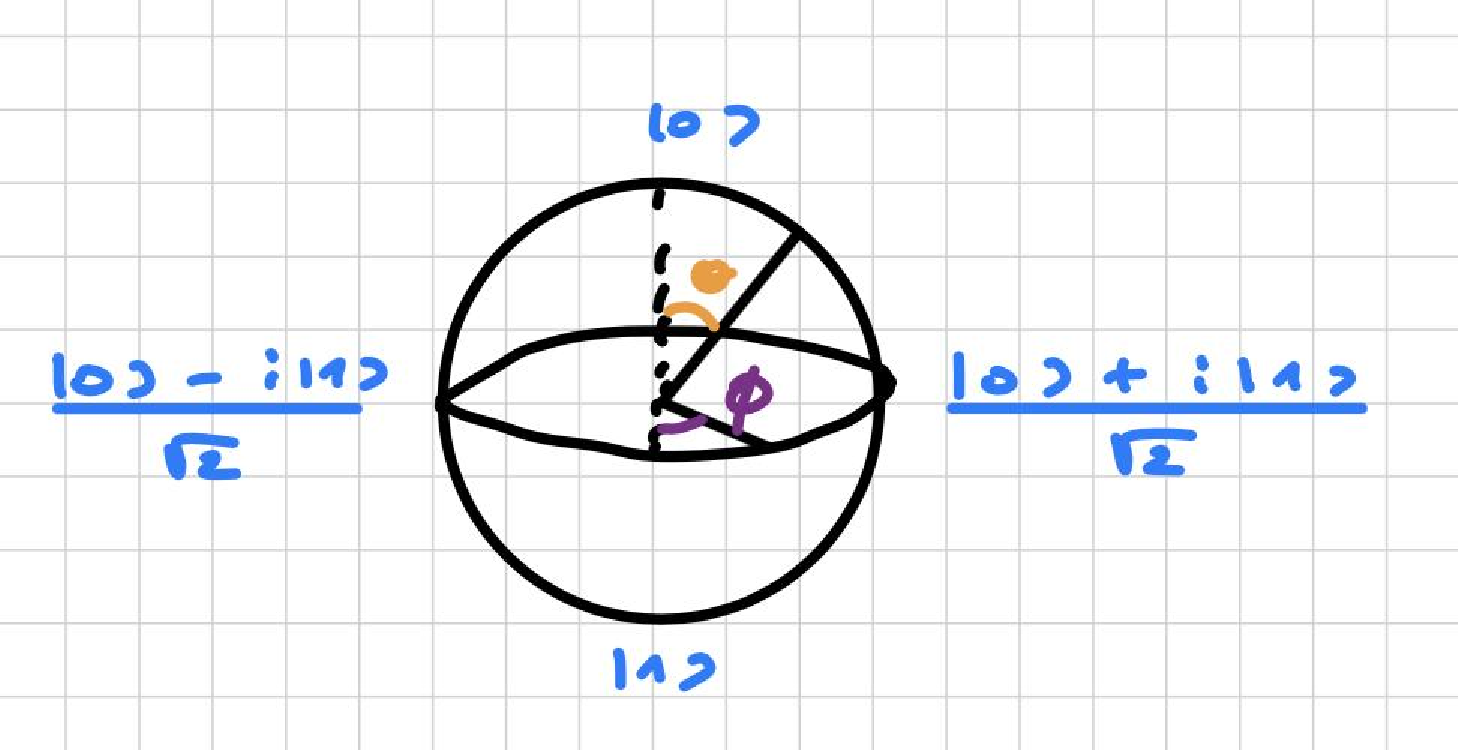
\includegraphics[width=0.6\linewidth]{images_in_pdf/16-/Grafico_97.pdf}
    \caption{Bloch sphere}
\end{figure}

\hl{We will interpret $\ket{0}$ and $\ket{1}$ as our polarized states $\ket{H}$ and $\ket{V}$}. In classical optics we have an unitary sphere to represent polarized states called \textbf{Poincaré sphere}: 
\begin{figure}[H]
    \centering
    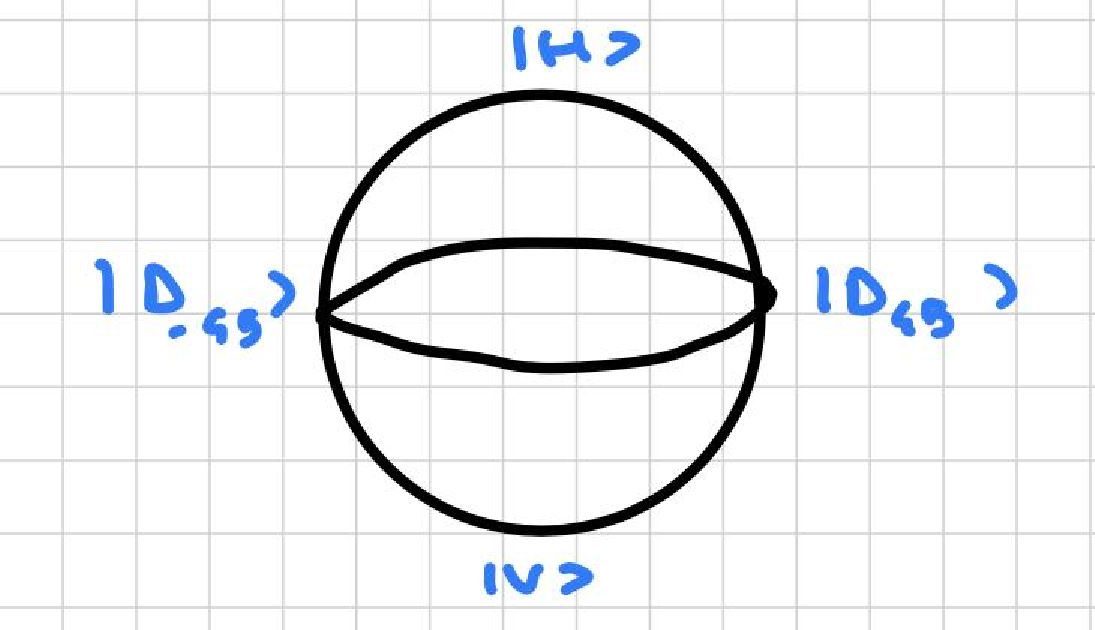
\includegraphics[width=0.6\linewidth]{images_in_pdf/16-/Grafico_98.pdf}
    \caption{Poincaré sphere}
\end{figure}

In this way, 2 bits become 2 qubits:
\begin{equation}\label{eqn:16-two-qubits-state}
00,01,10,11 \implies \ket{\psi} = a\, \ket{0}\ket{0}+ b\, \ket{0}\ket{1}+ c\, \ket{1}\ket{0}+ d\, \ket{1}\ket{1}
\end{equation}

A frequently used set of 2 qubits states are the \textbf{Bell states}, both entangled:
\begin{equation}\label{eqn:16-bell-states}
\ket{\phi^{\pm}} = 
\frac{1}{\sqrt{2}}\, 
\bigl(
    \ket{0}\ket{0}\pm \ket{1}\ket{1}
\bigr)
\hspace{2ex} \land \hspace{2ex}
\ket{\psi^{\pm}} =
\frac{1}{\sqrt{2}}\, 
\bigl(
    \ket{0}\ket{1}\pm \ket{1}\ket{0}
\bigr)
\end{equation}

We need to remember two important things:
\begin{enumerate}
    \item Classical information channels implies that the information can't be faster than the speed of light velocity $C$;
    
    \item We need to remember that there is the \textbf{no cloning theorem}.
\end{enumerate}

\begin{figure}[H]
    \centering
    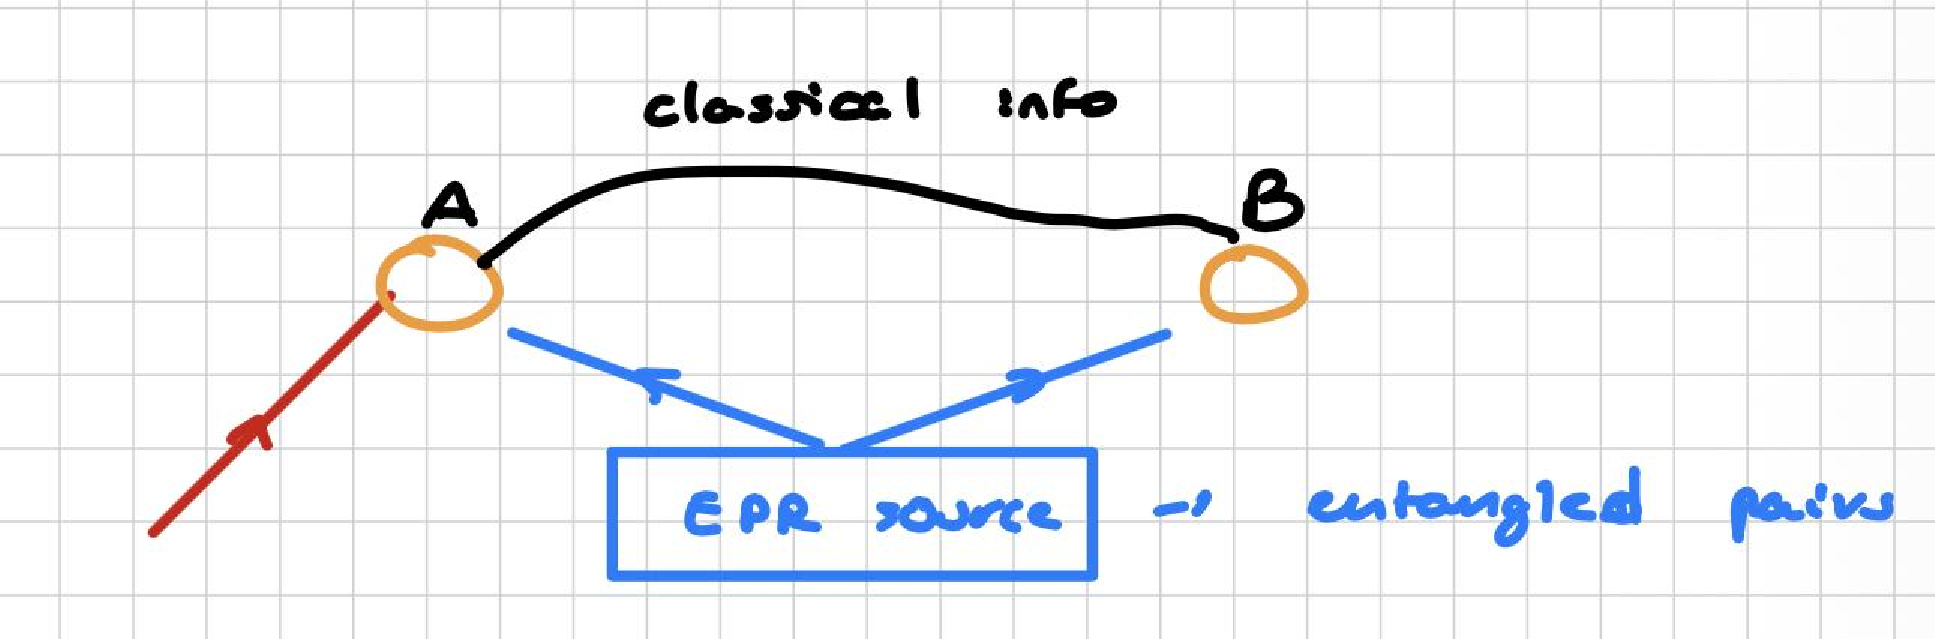
\includegraphics[width=0.6\linewidth]{images_in_pdf/16-/Grafico_99.pdf}
    \caption{Simple scheme of the teleportation protocol}
\end{figure}

\subsubsection{Teleportation protocol}

Suppose Alice has a photon in a particular state $\ket{\psi_A}$ that she wants to teleport to Bob:
\begin{equation}\label{eqn:16-teleportation-initial-state}
\ket{\psi_A} =c_0\, \ket{0}_A +c_1 \, \ket{1}_A.
\end{equation}

In the following, kets will always indicate -- by pedice $A$ or $B$ -- their respective owner. Alice may not know $c_0$ and $c_1$, but she can communicate with Bob through a classical channel. Then \hl{we have a EPR source which send separately entangled photons to Alice and Bob}:
\begin{equation}\label{eqn:16-epr-source}
\ket{\varphi_{AB}} =\frac{1}{\sqrt{2}}\, 
\bigl(
    \ket{0}_A\ket{0}_B+\ket{1}_A\ket{1}_B
\bigr).
\end{equation}

We consider the 3-photon state as:
\begin{equation}\label{eqn:16-teleportation-initial-state-2}
\ket{\Psi} = \ket{\varphi_{AB}}\,\ket{\psi_A} = 
\frac{1}{\sqrt{2}}\, 
\bigl(
    \ket{0}_A\ket{0}_B+\ket{1}_A\ket{1}_B
\bigr)
\, 
\bigl(
    c_0\, \ket{0}_A +c_1 \, \ket{1}_A
\bigr)
\end{equation}

If we consider the Bell (already defined in Equation \ref{eqn:16-bell-states}) states only using Alice's photons:
\begin{equation}\label{eqn:16-bell-states-alice}
\ket{\phi^{\pm}}_{AA} = 
\frac{1}{\sqrt{2}}\, 
\bigl(
    \ket{0}_A\ket{0}_A\pm\ket{1}_A\ket{1}_A
\bigr) 
\hspace{2ex} \land \hspace{2ex}
\ket{\psi^{\pm}}_{AA} = 
\frac{1}{\sqrt{2}}\, 
\bigl(
    \ket{0}_A\ket{1}_A\pm\ket{1}_A\ket{0}_A
\bigr) 
\end{equation}

Using them we can rewrite the \textbf{total 3-qubit state} as:
\begin{align}
\ket{\Psi} &= 
\ket{\psi}_A \otimes \ket{\varphi}_{AB} = \nonumber \\[0.5ex]
&= \frac{1}{\sqrt{2}} 
\bigl[ 
    c_0\ket{0}_A\ket{0}_A\ket{0}_B + 
    c_0\ket{0}_A\ket{1}_A\ket{1}_B + \nonumber \\[0.5ex]
    &\qquad +
    c_1\ket{1}_A\ket{0}_A\ket{0}_B +
    c_1\ket{1}_A\ket{1}_A\ket{1}_B 
\bigr] = \nonumber \\[0.5ex]
&= \frac{1}{2} 
\bigl[ 
    \ket{\phi^+}_{AA} 
    \left(c_0\ket{0}_B + c_1\ket{1}_B\right) + 
    \ket{\phi^-}_{AA}
    \left(c_0\ket{0}_B - c_1\ket{1}_B\right) + \nonumber \\[0.5ex]
    &\qquad + 
    \ket{\psi^+}_{AA} 
    \left(c_0\ket{1}_B + c_1\ket{0}_B\right) +
    \ket{\psi^-}_{AA} 
    \left(c_0\ket{1}_B - c_1\ket{0}_B\right) 
\bigr]. \label{eqn:quantum-teleportation-algebra}
\end{align}

\calloutinfo{%}
Notice that Alice and Bob have sufficient information to write this expression. To any possible outcome of Alice's measurement, there is a corresponding state of Bob's photon. The measurement on Alice's side constrains the state of Bob's photon into one of four possible states, each related to Alice's original state $\ket{\psi_A}$ by a known unitary transformation.
}

\subsubsection{Teleportation protocol: all possible scenarios unpacked}

In the following, we unpack all the possible scenarios after Alice performs a measurement on the Bell basis:
\begin{enumerate}
    \item \textbf{Alice obtains $\ket{\phi^+}$}: after projecting on the ket, Bob will obtain a copy of Alice's initial photon state:
    \begin{equation}\label{eqn:16-bob-state-alice-phi-plus}
        c_0\, \ket{0}_B+c_1\, \ket{1}_B
    \end{equation}

    Alice communicates to Bob -- through the classical channel -- her result and \hl{Bob instantly knows his photon is in state $\ket{\psi_A}$ without needing to measure the state}, so we actually made the teleportation.

    \item \textbf{Alice obtains $\ket{\phi^-}$}: after projecting on the ket, Alice tells her measurement result to Bob; he will immediately know that his photon is in the state:
    \begin{equation}\label{eqn:16-bob-state-alice-phi-minus}
        c_0\, \ket{0}_B-c_1\, \ket{1}_B
    \end{equation}

    To resolve it Bob changes the sign by applying a \textbf{unitary operation} to his photon; this is a \hl{polarization rotation by a half-wave plate}:
    \begin{equation}\label{eqn:16-bob-state-alice-phi-minus-transformation}
        \ket{0}_B \to \ket{0}_B \hspace{1cm} \ket{1}_B \to -\ket{1}_B
    \end{equation}
    
    \item \textbf{Alice obtains $\ket{\psi^+}$}: after projecting on the ket, Bob will know that his photon is in the state:
    \begin{equation}\label{eqn:16-bob-state-alice-psi-plus}
        c_0\, \ket{1}_B+c_1\, \ket{0}_B
    \end{equation}

    To resolve it Bob changes the sign by applying a \textbf{unitary operation} to his photon:
    \begin{equation}\label{eqn:16-bob-state-alice-psi-plus-transformation}
        \ket{1}_B \to \ket{0}_B \hspace{1cm} \ket{0}_B \to \ket{1}_B
    \end{equation}

    \item \textbf{Alice obtains $\ket{\psi^-}$}: after projecting on the ket, Bob will know that his photon is in the state:
    \begin{equation}\label{eqn:16-bob-state-alice-psi-minus}
        c_0\, \ket{1}_B-c_1\, \ket{0}_B
    \end{equation}

    To resolve it Bob changes the sign by applying a \textbf{unitary operation} to his photon:
    \begin{equation}\label{eqn:16-bob-state-alice-psi-minus-transformation}
        \ket{1}_B \to \ket{0}_B \hspace{1cm} \ket{0}_B \to -\ket{1}_B
    \end{equation}

\end{enumerate}

All the beforehand mentioned operations are $2\times2$ unitary matrices; it is possible to show that such matrices are generated by a four-element set $\left\{ \identity, \sigma_x,\sigma_y,\sigma_z\right\}$ comprising Pauli matrices and the identity matrix:
\begin{equation}\label{eqn:16-span-pauli-matrices}
    U = 
    \alpha_1 \sigma_x + \alpha_2 \sigma_y + \alpha_3 \sigma_z + \beta \identity
    \equiv
    \vec{\alpha} \cdot \vec{\sigma} + \beta \identity;
    \hspace{2ex}
    \forall\,
    U\ s.t.\ U^\dagger = U^{-1};
    \hspace{2ex}
    \vec{\alpha}\in\mathbb{C}^3,\, \beta\in\mathbb{C}.
\end{equation}

\calloutinfo{%}
    Notice that \textbf{there is no violation of the no-cloning theorem}, because the Bell-state \textbf{measurement destroys the original state} during the teleportation process.
}

\subsection{Experimental setup of the Innsbruck group}
The experiment starts with a UV pump beam exciting a nonlinear crystal, which acts as an EPR source and produces an entangled photon pair, this time labelled 2 and 3, in the Bell state
\begin{equation}\label{eqn:16-innsbruck-epr-pair}
\ket{\psi^-}_{2,3}=\frac{1}{\sqrt{2}}
\left(\ket{H}_2\ket{V}_3-\ket{V}_2\ket{H}_3\right).
\end{equation}

In this state, the two photons do not have a definite polarization individually, but only as a joint system. A second UV pump beam, reflected by a mirror, generates another photon pair; one photon is used as a trigger to synchronize the experiment, while the other -- referred to as photon 1 -- is prepared in an arbitrary polarization state,
\begin{equation}\label{eqn:16-innsbruck-state-to-teleport}
\ket{\psi}_1 =
\alpha\ket{0}_1+\beta\ket{1}_1,
\end{equation}

which is the unknown state to be teleported. Alice then performs a Bell-state measurement on photons 1 and 2 by sending them to a beam splitter followed by two detectors.
\begin{figure}[H]
    \centering
    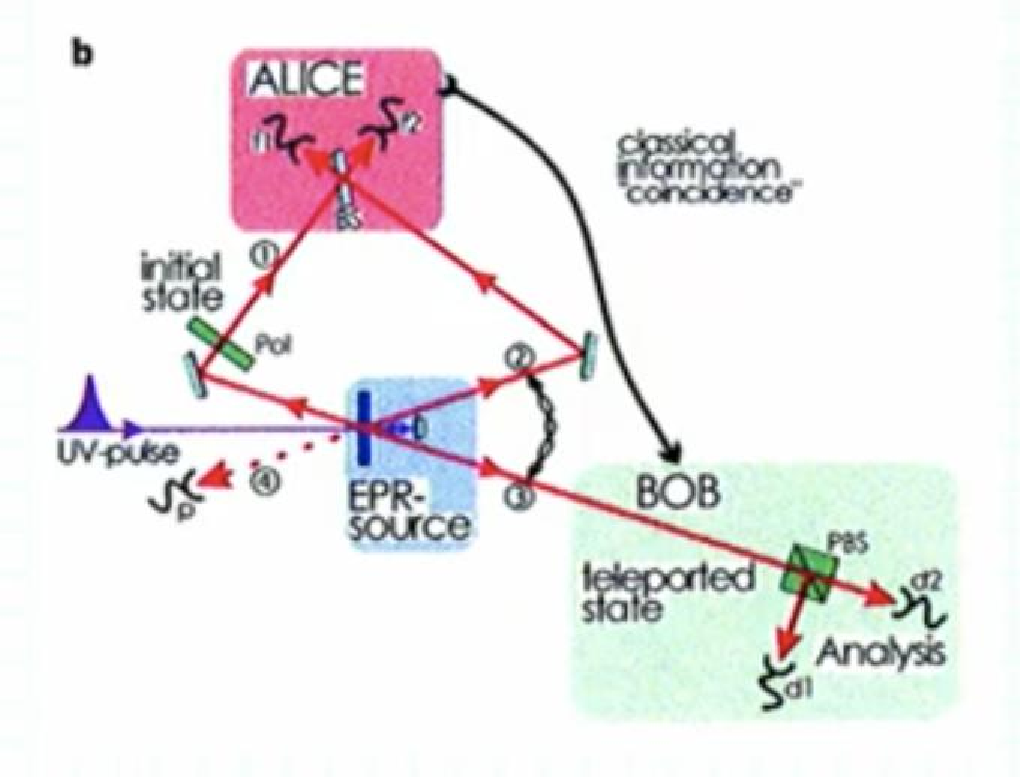
\includegraphics[width=0.6\linewidth]{images_in_pdf/16-/Grafico_100.pdf}
    \caption{Experimental setup for teleportation of the Innsbruck group.}
\end{figure}

\hl{In this implementation, the Bell state $\ket{\psi^-}_{1,2}$ is the easiest one to identify, because it \textbf{is the only state that produces coincidence counts} at the two detectors after the beam splitter}, whereas the other Bell states are symmetric under exchange and therefore lead to bunching at the same output port. The reason is that $\ket{\psi^-}_{1,2}$ is \textbf{antisymmetric under particle exchange}, so the two photons must exit through different output ports, giving simultaneous clicks. If Alice detects $\ket{\psi^-}_{1,2}$, then photon 3 is projected onto the same state that photon 1 initially carried, up to a known phase depending on the chosen convention,
\begin{equation}\label{eqn:16-innsbruck-teleported-state}
\ket{\psi}_3 \sim
\alpha \ket{0}_B+ \beta \ket{1}_B.
\end{equation}

In this sense, the Bell-state measurement destroys the identity of photon 1 during the process, so the state is not copied but transferred to Bob's photon, in full agreement with the no-cloning theorem. \hl{The key point is that photons 2 and 3 were initially prepared in the entangled state $\ket{\psi^-}_{2,3}$}, so the measurement on photons 1 and 2 effectively teleports the quantum information from photon 1 to photon 3. 

\calloutinfo{%
    Bob can then verify the success of the teleportation by analyzing the polarization of his photon with a polarizing beam splitter set at $+45^\circ$ and $-45^\circ$, and by measuring the corresponding coincidence counts at detectors $D_3$ and $D_4$.
}

Further readings are: \cite{art:Ursin-2007-144km-teleportation}, \cite{art:Wang-2017-ground-to-satellite} and \cite{art:Yin-2020-entanglement-based-crypto}.

\subsection{Entanglement swapping}

At this stage we only know how to create entanglement between photons generated by the same source.

\question{Can entanglement also be distributed between particles that come from different sources and have never interacted?}{%
The answer is yes: this is the idea of \textbf{entanglement swapping}. A Bell-state measurement on two photons can transfer entanglement to the remaining two photons, even if they are far apart and originate from independent sources.
}

We consider two different EPR sources emitting the entangled pairs $(1,2)$ and $(3,4)$. The four-photon state is
\begin{equation}\label{eqn:16-entanglement-swapping-epr-pairs-couple}
\ket{\psi}_{1,2,3,4}
=
\frac{1}{2}
\bigl(\ket{H}_1\ket{V}_2-\ket{V}_1\ket{H}_2\bigr)
\otimes
\bigl(\ket{H}_3\ket{V}_4-\ket{V}_3\ket{H}_4\bigr).
\end{equation}

The first factor describes the entanglement between photons 1 and 2, while the second factor describes the entanglement between photons 3 and 4. Their product means that there is initially no entanglement between the two pairs.
\begin{figure}[H]
    \centering
    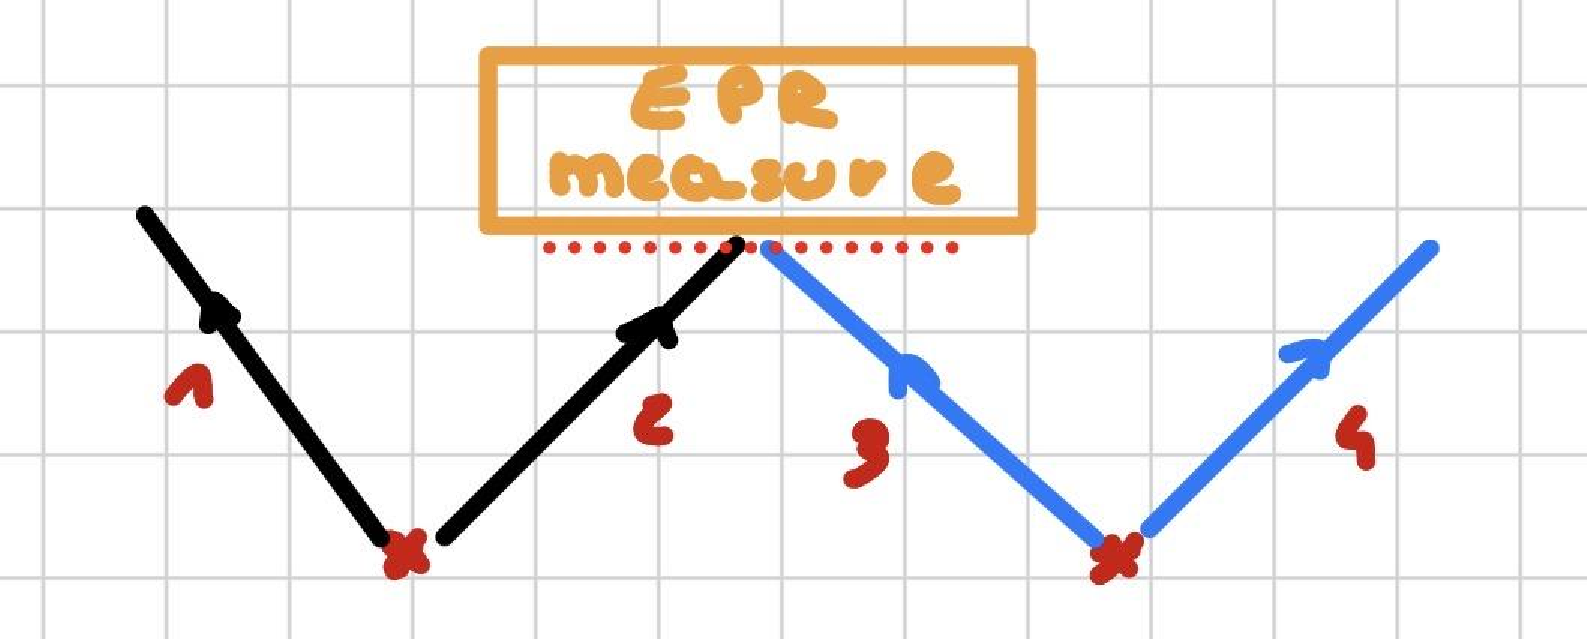
\includegraphics[width=0.6\linewidth]{images_in_pdf/16-/Grafico_101.pdf}
    \caption{Scheme of entanglement swapping in a quantum repeater.}
\end{figure}

The Bell states of photons 2 and 3 are
\begin{align}
\ket{\psi^{\pm}}_{2,3}
&= \frac{1}{\sqrt{2}}
\bigl(
    \ket{H}_2\ket{V}_3\pm\ket{V}_2\ket{H}_3
\bigr),
\\
\ket{\phi^{\pm}}_{2,3}
&= \frac{1}{\sqrt{2}}
\bigl(
    \ket{H}_2\ket{H}_3\pm\ket{V}_2\ket{V}_3
\bigr).
\end{align}

Using these definitions, the initial four-photon state can be rewritten as
\[
\ket{\psi}_{1,2,3,4} = \frac{1}{2}\, \left(\ket{\psi^+}_{1,4}\ket{\psi^+}_{2,3}+\ket{\psi^-}_{1,4}\ket{\psi^-}_{2,3}+\ket{\phi^+}_{1,4}\ket{\phi^+}_{2,3}+\ket{\phi^-}_{1,4}\ket{\phi^-}_{2,3}\right)
\]

\calloutinfo{%
    Therefore, a Bell-state measurement on photons 2 and 3 projects photons 1 and 4 onto the corresponding Bell state. In particular, if photons 2 and 3 are found in the state $\ket{\psi^-}_{2,3}$, then photons 1 and 4 are projected onto \(\ket{\psi^-}_{1,4}\). \textbf{This means that entanglement has been swapped}: photons 1 and 4 become entangled even though they never interacted directly.
}

Notice that we need to fulfill specific conditions:
\begin{itemize}
    \item They come from different sources;
    \item They never interacted ;
    \item The entangled state of 1 and 4 is exactly the same of the entangled state 2 and 3.
\end{itemize}

\textbf{Experimentally}, \hl{one looks for coincidences between the detectors $D_1^\dagger $ and $D_4$, or between $D_1^-$ and $D_4$}, conditioned on the detection of $\ket{\psi^-}_{2,3}$. Photon 1 is analyzed along the $+45^\circ$ and $-45^\circ$ bases, while photon 4 is analyzed at a variable polarization angle $\theta$. \hl{If entanglement swapping occurs, the coincidence rate for one analyzer setting reaches a minimum while the complementary setting reaches a maximum}, exactly as expected for an entangled Bell pair.

Looking at the coincidence rates as a function of $\theta$ in Figure \ref{16-entanglement-swapping}, one finds that:
\begin{itemize}
    \item $D_1^\dagger -D_4$ coincidence rate for  $\theta =+ 45^\circ\implies $ is Min
    \item $D_1^--D_4$ coincidence rate for  $\theta =+ 45^\circ\implies $ is Max 
\end{itemize}

\begin{figure}[H]
    \centering
    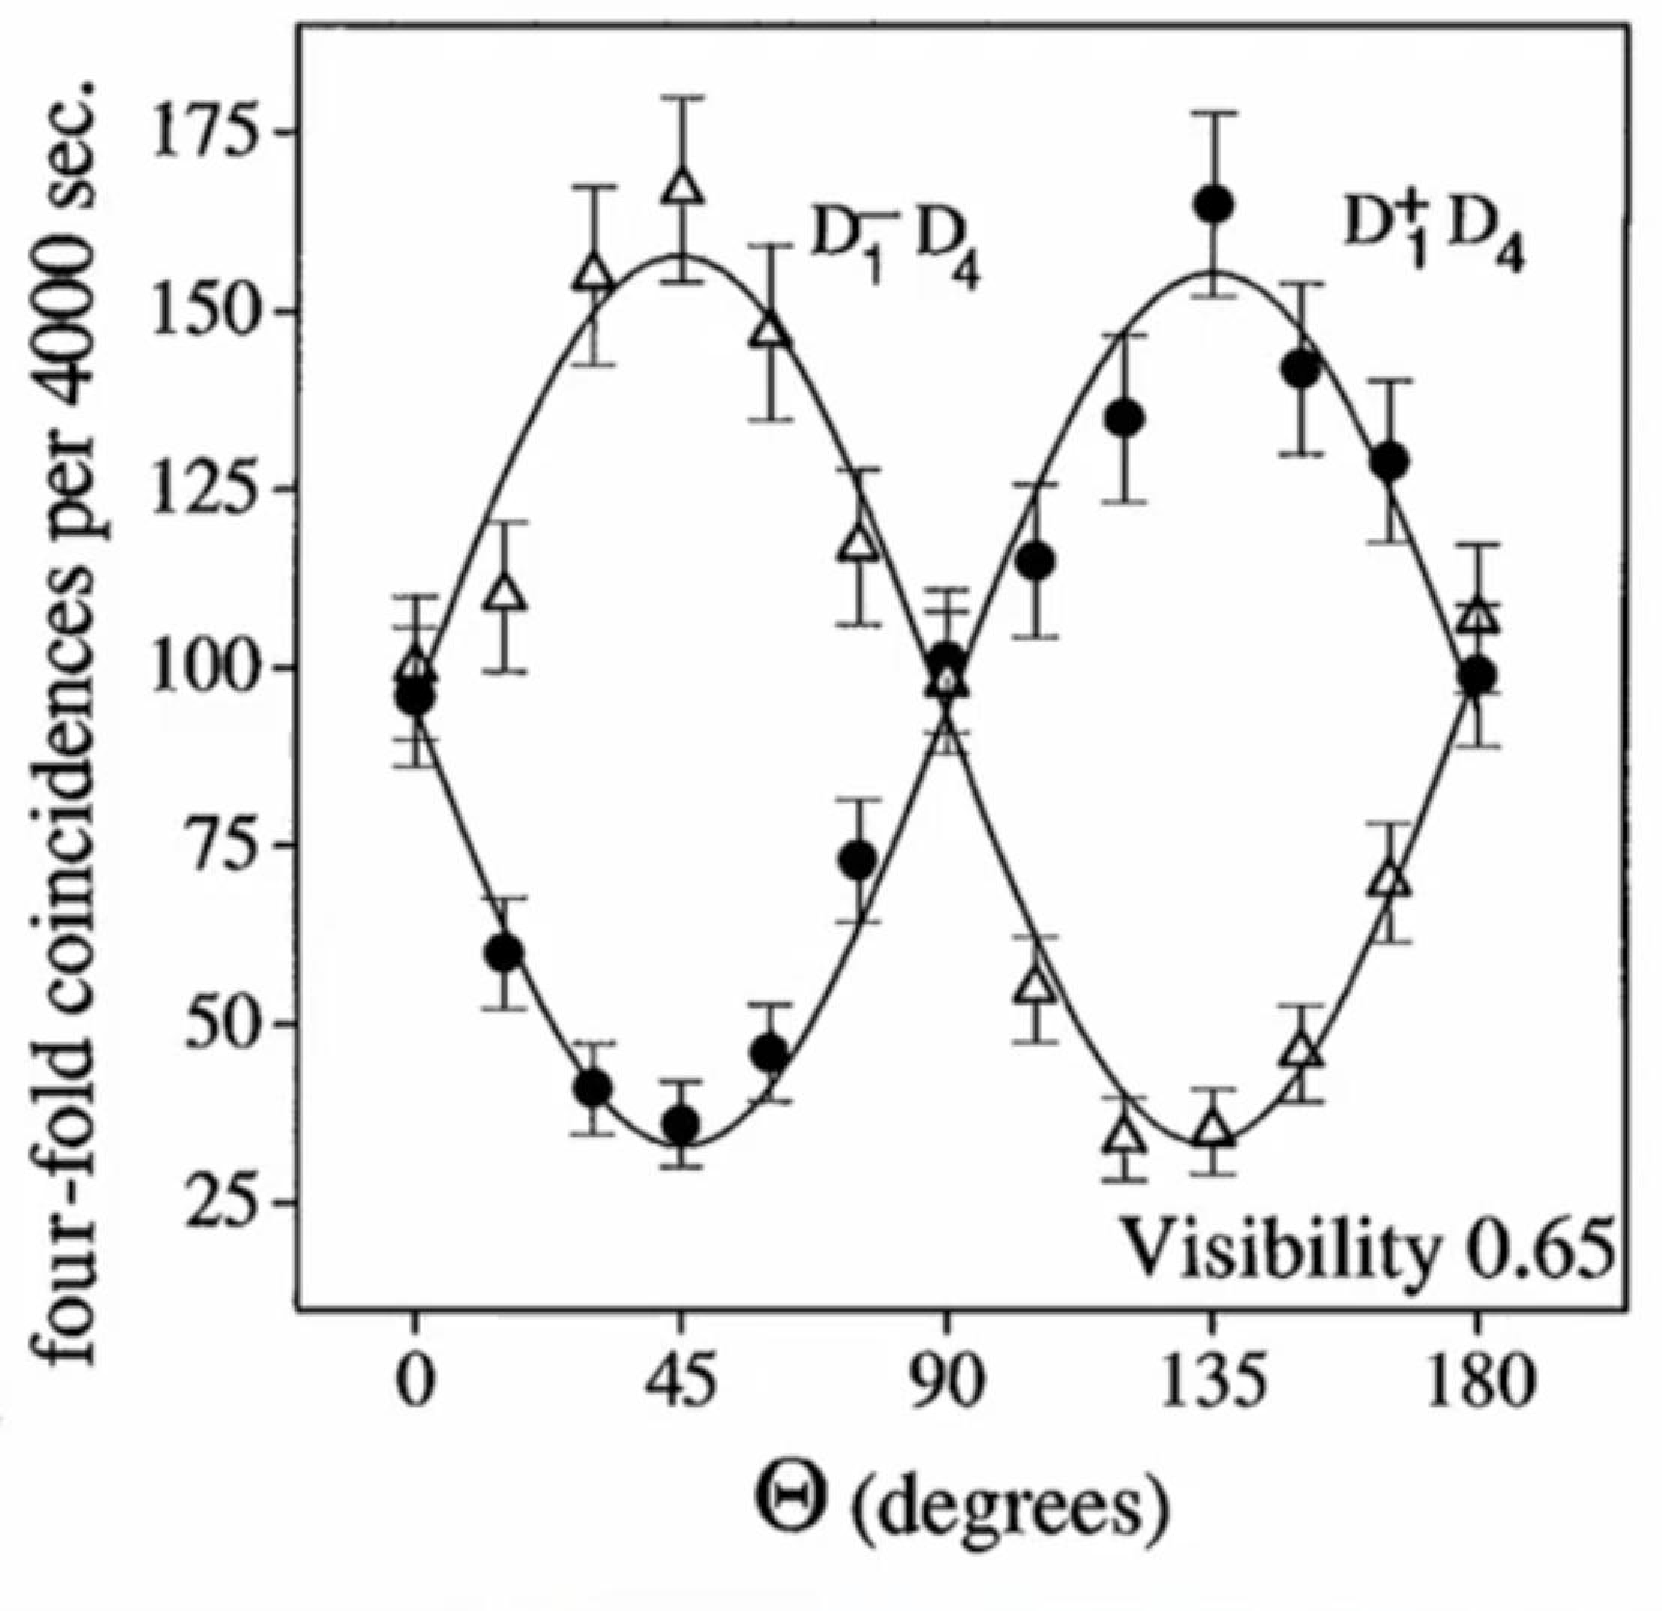
\includegraphics[width=0.6\linewidth]{images_in_pdf/16-/Grafico_102.pdf}
    \caption{Coincidence rates for entanglement swapping.}
    \label{16-entanglement-swapping}
\end{figure}

In this way, entanglement is not created by direct interaction between photons 1 and 4, but is heralded by the Bell-state measurement performed on photons 2 and 3.
Notice that there is no violation of the no-cloning theorem, because in the process of performing the Bell state measurement, \hl{the original state is itself destroyed}.

\subsection{Quantum networks}

\hl{The idea of entanglement swapping can be extended to the propagation of entanglement across many nodes}. If the same scheme is replicated for $N$ sources, the entanglement can be distributed step by step so that the first photon becomes eventually entangled with the last one. In this way, entanglement is not simply transmitted, but propagated through a network, and this \hl{can be exploited for quantum communication tasks} such as \textbf{entanglement-based quantum key distribution} or the \textbf{connection of distant quantum processors}. 

Quantum information is generated, processed, and stored locally in quantum nodes, while the nodes are linked by quantum channels that transport quantum states from site to site with high fidelity and distribute entanglement over the whole network. The natural extension of this idea is the \textbf{quantum internet}.

\subsubsection{Quantum repeaters}

In a classical communication link, losses due to absorption, scattering, and other imperfections are usually compensated by repeaters or amplifiers, which restore the signal by copying the same information. In quantum communication this is impossible, because quantum states cannot be cloned. For this reason, one needs radically new hardware, namely \textbf{quantum repeaters}, in order to build a quantum internet. In their simplest form, \hl{quantum repeaters rely on entanglement swapping}:
\begin{enumerate}
    \item The repeater first generates entanglement with two neighboring nodes, whose distance from the repeater must be short enough to allow efficient transmission through a telecom channel.
    \begin{figure}[H]
        \centering
        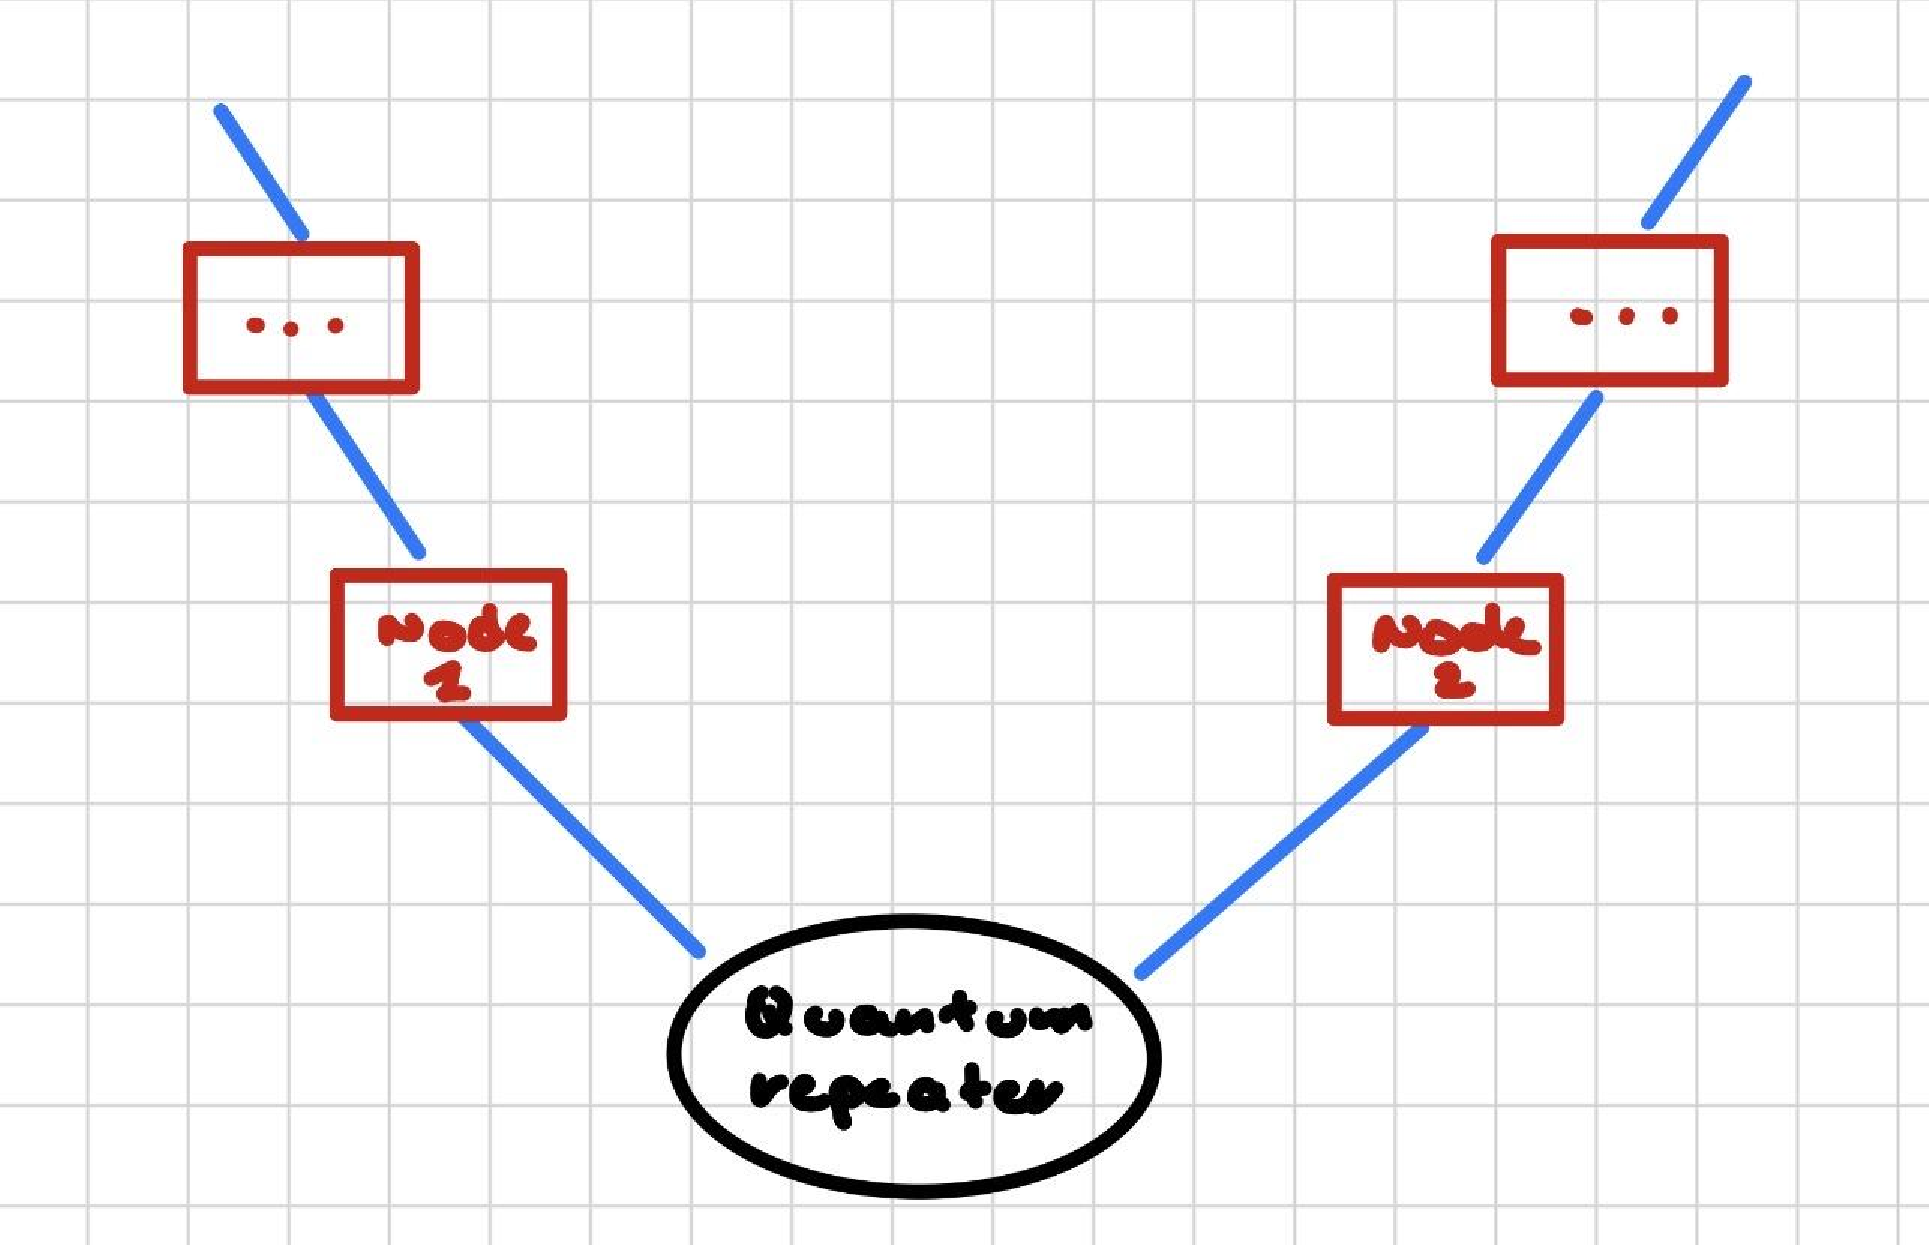
\includegraphics[width=0.6\linewidth]{images_in_pdf/16-/Grafico_103.pdf}
        \caption{Entanglement swapping in a quantum repeater.}
    \end{figure}

    \item The repeater then stores the quantum state for the time needed to establish entanglement with the next nodes in the network. This requires a \textbf{quantum memory}, which can be implemented, for instance, using long-lived spin degrees of freedom such as nuclear spins.

    \item To transmit information through a quantum network without losing coherence, a major direction of research focuses on spin-photon interfaces. These interfaces allow a quantum memory to herald the arrival of a photon and to store the associated quantum state. In this way, photon losses during transmission can be mitigated, and the stored state can later be retrieved on demand by emitting a photon carrying the same quantum information.

    A single-photon detector converts the arrival of a photon into an electrical signal, but the actual implementation of a spin-photon interface requires a much more specialized device. In semiconductor heterostructures, such as Si/Ge platforms, a two-dimensional electron gas can be formed and locally confined by electrostatic gates, creating quantum dots with single-electron control. These structures make it possible to manipulate electron spins, to store quantum information, and, in principle, to interface spin qubits with photons for teleportation, entanglement distribution, or quantum networking. However, such devices are technologically very demanding, and the realization of efficient single-photon sources and robust spin-photon interfaces remains a major experimental challenge.
\end{enumerate}